\chapter{The Standard Model of Particle Physics and beyond}
\label{chapter:SM}

The \acrfull{SMlabel} of particle physics~\cite{PhysRevLett.19.1264,GLASHOW1961579,RevModPhys.52.525} is the theoretical framework
that so far best describes subatomic particles and their interactions.
It is a \acrlongpl{QFT} (\acrshort{QFT}) and since its initial development in the 1960s,
the model has been overwhelmingly successful, guiding many experimental achievements
including the discovery of the top quark~\cite{topsearch1995,PhysRevLett.74.2626} in 1995
and the Higgs boson at the Large Hadron Colliders (LHC) in 2012~\cite{ATLASHiggs2012,CMShiggs2012}.
Despite its success, there are known phenomena not accounted for by the model
and questions which clearly point to the need of a new theory.\\

This chapter starts with an overview of the \acrshort{SMlabel}, building it with its mathematical formalism, and presenting a summary of the particle content and their interactions. Then, it continues with a summary of the current success of the theory,including its shortcomings and alternative models. The focus is given to models that include charged Higgs bosons or top FCNC interactions involving a scalar.\\

Throughout this dissertation, natural units are used: the speed of light and the reduced Planck constant are set to unity ($c=\hbar=1$),
electric charges are expressed in units of the electron electric charge ($-e$) and masses are expressed in terms of energy (eV). Throughout this chapter's theoretical developments, the Einstein summation convention is used by default.

\section{The \acrlong{SMlabel} of Particle Physics}

From the mathematical point of view, the \acrshort{SMlabel} is a renormalisable non-abelian gauge \acrshort{QFT} based on the
symmetry group, 

\begin{equation}
    \label{Theory_eq:SMgroup}
    SU(3)_C\otimes SU(2)_L\otimes U(1)_Y,
\end{equation}

where $SU(3)_C$ is the group described by \acrlongpl{QCD}~(\acrshort{QCD})~\cite{QCD} that
represents the strong interactions of coloured quarks and gluons (strong force),
while $SU(2)_L\times U(1)_Y$ is the inclusive representation of both electromagnetic (EM) and weak interactions
described by the \acrlongpl{EW}~(\acrshort{EW}) theory~\cite{PhysRevLett.19.1264,Salam:1968rm,GLASHOW1961579}. The \acrshort{SMlabel} describes all the interactions between elementary
particles except gravity, for which no renormalisable \acrshort{QFT} has been formulated so far.
The following sections introduce the particles of the \acrshort{SMlabel} and the theories that describe their interactions.  

\subsection{Particle content of the \acrlong{SMlabel}}

In the \acrshort{SMlabel}, elementary particles are described as excitations of quantum fields.
There are two main classes of particles within the theory: \textit{fermions} and \textit{bosons}.
The main difference between the two is the spin: fermions have half-integer spin and therefore obey the Pauli exclusion
principle~\cite{Pauli1925}, while bosons have integer spin.

\subsubsection{Fermions}

Fermions can be divided further into two categories: quarks and leptons, based on their interactions, or their charges.
Both types manifest in \acrshort{EW} interactions, having a weak isospin $T_3=\pm1/2$ while only the quarks experience the strong interaction. Quarks have a fractional electric charge $\abs{Q}=2/3$ or $1/3$, and the \textit{colour} charge. The last one is the charge associated to the strong interaction and its value is denoted as \textit{red}, \textit{green} and \textit{blue}. Table~\ref{tabSM:fermionscontent} presents a summary of the fundamental fermions.\\

\begin{table}[htbp]
    \begin{tabular}{ccccc}
    \toprule\toprule
    Generation & Name & Symbol & Mass & Charge \\ \midrule
    \multicolumn{5}{c}{Quarks}                          \\ \midrule
    \multirow{2}{*}{1\ts{st}}       & Up       &  $u$      &  $2.15^{+0.49}_{-0.26}$~MeV    &  $+2/3$ \\
                                    & Down     &  $d$      &  $4.67^{+0.48}_{-0.17}$~MeV    &  $-1/3$ \\
    \multirow{2}{*}{2\ts{nd}}       & Charm    &  $c$      &  $1.27\pm 0.02$~GeV            &  $+2/3$ \\
                                    & Strange  &  $s$      &  $93.4^{+8.6}_{-3.4}$~MeV      &  $-1/3$ \\
    \multirow{2}{*}{3\ts{rd}}       & Top      &  $t$      &  $172.69\pm 0.30$~GeV          &  $+2/3$ \\
                                    & Bottom   &  $b$      &  $4.18^{+0.03}_{-0.02}$~GeV    &  $-1/3$ \\
    \midrule
    \multicolumn{5}{c}{Leptons}                          \\ \midrule
    \multirow{2}{*}{1\ts{st}}       & Electron             &  $e^-$        &  $0.511$~MeV            &  $-1$ \\
                                    & Electron neutrino    &  $\nu_e$    &  $<1.1$~eV 90\% CL      &  $0$  \\
    \multirow{2}{*}{2\ts{nd}}       & Muon                 &  $\mu^-$      &  $0.106$~GeV            &  $-1$ \\
                                    & Muon neutrino        &  $\nu_\mu$  &  $<0.19$~MeV 90\% CL    &  $0$  \\
    \multirow{2}{*}{3\ts{rd}}       & Tau                  &  $\tau^-$     &  $1776.86\pm 0.12$~MeV  &  $-1$ \\
                                    & Tau neutrino         &  $\nu_\tau$ &  $<18.2$~MeV 95\% CL    &  $0$  \\

    \bottomrule\bottomrule
    \end{tabular}
    \caption{Table of the different quarks and leptons of the \acrshort{SMlabel} grouped in families with their mass and electric charge according to the Particle Data Group~\cite{pdg}. The uncertainties on the electron and the muon masses are below $10^{-10}$ and $10^{-6}$~MeV, respectively. The anti-matter states are not shown. }
    \label{tabSM:fermionscontent}
    \end{table}

There are a total of six quark types, named \textit{flavours}, and are split into three generations.
The first generation consists in the \textit{up} and the \textit{down} quark, the former with $Q=+2/3$ and $T_3=+1/2$,
while the latter $Q=-1/3$, $T_3=-1/2$ and a different mass.
The next two generations are copies of the first one with increasing mass, with a pair of \textit{up}-type and \textit{down}-type quarks.
The second generation consists in \textit{charm} and \textit{strange} quarks, and the third one in \textit{top} and \textit{bottom} quarks.
In addition, all the six quark flavours have anti-matter states with the same mass, but opposite quantum numbers. As an example,
an anti-\textit{up}-type quark has $Q=-2/3$, $T_3=-1/2$ and carries anti-\textit{red} colour.\\

Leptons are also similarly divided into six different types and in three separate generations named \textit{electron} ($e$), \textit{muon} ($\mu$) and \textit{tau} ($\tau$), also with increasing mass.
Each generation contains a lepton with $Q=-1$ and $T_3=+1/2$ named after its generation,
and an associated electrically neutral lepton with $T_3=-1/2$ named neutrino ($\nu$).
The neutrino is assumed to be massless in the formulation of the \acrshort{SMlabel},
however the phenomena of neutrino oscillations is an experimental proof of these particles actually having very small, but non-zero, mass values.
This apparent failure of the theory is discussed in Section~\ref{subsec:openquestions}. In the case of quarks, the associated anti-matter states have the same mass but opposite quantum numbers.\\

All the stable \acrshort{SMlabel} matter in the universe is constituted by the massive particles of the first generations of quarks and leptons, as the heavier versions eventually decay to lighter ones through their interactions. While it is possible to observe free leptons, quarks exist only in bound states, or hadrons, like the neutron or the proton. This is a feature of the strong interaction called confinement, discussed in Section~\ref{subsec:QCD}. Only colour-less bounded states of quarks are observable, and can be built from three quarks with overall half-integer spin, named baryons, or by two quarks with integer spin, named mesons.\\

In the context of particle physics, the formulation of the classical Lagrangian, $\mathcal{L}$, is used to describe physics systems.
A generic free fermion field $\psi$ with mass $m$, can be described by the Dirac Lagrangian, 

\begin{equation}
\label{Theory_eq:diraceq}
    \mathcal{L} = \bar{\psi}(i\gamma^\mu\partial_\mu-m)\psi,
\end{equation}
where $\gamma^\mu$ are Dirac matrices and $\partial_\mu$ is the four-momentum derivative.

\subsubsection{Bosons}

Particles with integer spin are referred to as bosons. When the bosonic sector with spin 1 gauge fields are force carriers that naturally follow from imposing the requirement of local gauge invariance on Equation~\ref{Theory_eq:diraceq} under symmetry groups, in this case detailed in Equation~\ref{Theory_eq:SMgroup}. In Section~\ref{subsec:SMinteractions} the nature and origins of the gauge bosons are detailed. Table~\ref{tabSM:bosonscontent} presents a summary of the bosons of the \acrshort{SMlabel}.\\

\begin{table}[htbp]
    \begin{tabular}{ccccc}
    \toprule\toprule
    Name                  & Mass [GeV] & Charge & Interaction \\ \midrule
    Photon ($\gamma$)     &  0                             &  $0$ & Electromagnetic\\
    $Z$                   &  $91.1876 \pm 0.0021$~GeV      &  $0$ & \multirow{2}{*}{Weak} \\
    $W^\pm$               &  $80.377\pm 0.012$~GeV         &  $\pm 1$ & \\
    Gluon ($g$)           &  0                             &  0 & Strong \\
    Higgs                 &  $125.25\pm0.17$~GeV           &  0      & - \\
    \bottomrule\bottomrule
    \end{tabular}
    \caption{Table of the different bosons of the \acrshort{SMlabel} with their masses and electric charges according to the Particle Data Group~\cite{pdg}. The Higgs boson has spin 0 and does not mediate an interaction, while the rest have spin 1 and mediate an interaction.}
    \label{tabSM:bosonscontent}
    \end{table}

In summary, the photon ($\gamma$) is the carrier of the electromagnetic force, being a massless and electrically neutral particle.
The weak force carriers are the $W^+$, $W^-$ and $Z$ bosons, all massive with the $Z$ boson being electrically neutral and the $W^\pm$ with either $Q=\pm1$. Gluons ($g$) are the strong force carriers which are massless and with no electric charge. There are eight different gluons representing each possible colour exchange.\\

The \acrshort{SMlabel} also includes a neutral spin-0 particle, or \textit{scalar}, the Higgs boson. The Higgs field is responsible for all SM particles acquiring mass through the Higgs mechanism, as described in Section~\ref{subsec:SSB}.
The kinematics of a generic scalar $\phi$ with mass $m$, is described by the Klein-Gordon Lagrangian,

\begin{equation}
    \label{Theory_eq:KGeq}
    \mathcal{L}=\frac{1}{2}\partial^\mu\phi\partial_\mu\phi - m^2\phi^2.
\end{equation}

Charged scalars can be described instead through a complex field $\phi$ (with its complex conjugate $\phi^*$) and the expression of the Lagrangian is slightly modified,

\begin{equation}
    \label{Theory_eq:KGeqcharged}
    \mathcal{L}=\partial^\mu\phi\partial_\mu\phi^* - m^2\phi\phi^*.
\end{equation}

Vector fields $A^\mu$, which represent spin 1 bosons, are described by the Proca Lagrangian,

\begin{equation}
    \label{Theory_eq:Proca}
    \mathcal{L}=-\frac{1}{4}F^{\mu\nu}F_{\mu\nu}+\frac{1}{2}m^2A^\mu A_\mu,
\end{equation}
with $F^{\mu\nu}=\partial^\mu A_\nu -\partial^\nu A_\mu$ being the field strength tensor.
In the case of massless particles, the previous expression with $m=0$ is known as the Maxwell Lagrangian.

\subsection{Interactions of the Standard Model}
\label{subsec:SMinteractions}
The Lagrangian of the \acrshort{SMlabel} is defined to be locally invariant to the symmetry group in the Expression~\ref{Theory_eq:SMgroup},
condition that generates and defines the interactions of the corresponding particles as representations of the symmetry transformations.\\

For a generic Lagrangian, the physical system can have various symmetries, so its Lagrangian is invariant under different types of transformations.
These transformations can be either time-space independent, called global transformations, or dependent, called gauge or local transformations.
Any invariant transformation of a Lagrangian describes a physical system which conserves a physical quantity, as described by the Noether theorem~\cite{Noether}.
Then, the interactions are introduced in the Lagrangian as additional terms by promoting an already existing global symmetry, $\phi$,
of the Lagrangian to a local gauge symmetry, $\phi(x)$. The physical motivation behind introducing gauge symmetries
is to be able to describe vector bosons in \acrshort{QFT}.
The procedure expands the theory with additional fields that mediate the resulting interactions,
which properties depend on the characteristics of the symmetry group.\\

An example of the process is shown to afterwards derive the \acrshort{SMlabel} interactions of the strong and electroweak sectors. 

\subsubsection{Gauging a symmetry to interaction}

A general global transformation $\theta$ which acts upon the field $\psi$ is described as

\begin{equation}
    \psi\rightarrow e^{ig\theta^aT^a}\psi,
\end{equation}

with $g$ being the coupling constant and $T^a$ being the generators of the Lie group associated to the transformation (like $SU(n)$ or $U(n)$), with $a$ ranging from 1 to $n^2-1$, for $n>1$, and corresponding to the number of the Lie algebra..
The generators can be characterised by their commutation relation, 

\begin{equation}
\label{Theory_eq:nonabcomutator}
    [T^a,T^b]=if^{abc}T^c,
\end{equation}

where $f^{abc}$ are the structure constants of the group. Following Noether's theorem, there are as many conserved quantities as generators of the Lagrangian's symmetries. As an example, it is straightforward to see that a Lagrangian like the one in
Equation~\ref{Theory_eq:diraceq} is invariant to a $U(1)$ transformation where $\theta$ is just a constant and hence, a constant phase change.
One can obtain the current, $j^\mu$, as

\begin{equation}
    j^\mu = \bar{\psi}\gamma^\mu\psi,
\end{equation}

and is conserved, $\partial_\mu j^\mu = 0$, with the conserved charge,
\begin{equation}
Q=\int \mathrm{d}^3x j^0 = \int \mathrm{d}^3x\psi^{\dag}\psi. %= \int \frac{\mathrm{d}^3p}{(2\pi)^3}(a^\dag a - b^\dag b)
\end{equation}

%where the field has been expressed in an expansion over plane waves,

%\begin{equation}
%\psi(x)=\int\frac{\mathrm{d}^3k}{2\sqrt{8\pi^3(\textbf{k}^2+m^2)}}[a(\textbf{k})e^{-ikx}+b^\dag(k)e^{ikx}]
%\end{equation}
%with $a,b$ the Fock's space anihilation operators to the vacuum of two different particles. 

With some algebra and by introducing solutions in momentum space, $\psi$ can be interpreted as a fermion anihilation and an anti-fermion creation (the other way around with $\psi^\dag$) in the Fock space and then, the product becomes the difference of the number of fermion and anti-fermion leading to the conservation of the fermion number.\\

Promoting the global symmetry to a local symmetry is done by introducing locality in the $\theta$ transformation,
$\theta \rightarrow\theta(x)$, which introduces new $\partial_\mu\theta$ terms in the Lagrangian.
A way to balance the new terms and, hence, keep the Lagrangian invariant, is to introduce gauge vector fields $A_\mu^a$,
following the Yang-Mills theory~\cite{YangMills}. In the most generalised approach, there have to be as many $A_\mu^a$
as generators of the symmetry, which transform as,

\begin{equation}
    A_\mu^a \rightarrow A_\mu^a + \partial_\mu\theta^a + gf^{abc}A_\mu^b\theta^c.
\end{equation}

Note that the last term proportional to the structure constant and relates the gauge field to the conserved symmetry charge.
The next step is to replace the standard derivative in the Lagrangian by the covariant derivative,

\begin{equation}
    D_\mu\equiv\partial_\mu - igT^aA_\mu^a.
\end{equation}

The final ingredient is to complete the Lagrangian with the the kinematic Lagrangian for the massless vector fields,
the Maxwell Lagrangian from Equation~\ref{Theory_eq:Proca} with a slightly different field strength tensor,

\begin{equation}
    F_{\mu\nu}^a=\partial_\mu A_\nu^a - \partial_\nu A_\mu^a + gf^{abc}A_\mu^bA_\nu^c.
\end{equation}

The last term is present only for non-abelian symmetry groups, since it is proportional to the structure constants, and has big consequences in the resulting interactions, as discussed in the next section.
Another remark is that the gauge fields have to be massless, as a mass term proportional to $A_\mu^cA^{\mu c}$ is not gauge invariant.\\

As an example, the promotion of the global $U(1)$ symmetry in Equation~\ref{Theory_eq:diraceq} results in the upgraded Lagrangian,
\begin{equation}
\label{Theory_eq:diraceq20}
\begin{split}
    \mathcal{L}_{\ \ } &= \bar{\psi}(i\gamma^\mu D_\mu-m)\psi - \frac{1}{4}F_{\mu\nu}F^{\mu\nu} \\
    D_{\mu \ } &\equiv \partial_\mu -igA_\mu \\
    F_{\mu\nu} &\equiv \partial_\mu A_\nu - \partial_\nu A_\mu,
\end{split}
\end{equation}
after just one massless gauge field that interacts with the field $\psi$.
The interaction term between the two fields is $g\bar{\psi}\gamma^\mu A_\mu\psi$,
hidden in the covariant derivative definition and proportional to the coupling constant $g$.\\

The Lagrangian of the \acrshort{SMlabel} ($\mathcal{L}_{SM}$), is built from imposing local invariance under $SU(3)_C$ transformations,
which leads to strong interactions; and by imposing $SU(2)_L\times U(1)_Y$ transformations, which brings EW interactions. It can be written as
\begin{equation}
    \mathcal{L}_{SM} = \mathcal{L}_{QCD}+\mathcal{L}_{EW}.
\end{equation}

After this introduction on field theory, the theories of the two orthogonal sectors in the \acrshort{SMlabel} are described and followed by a description of the mechanism to introduce mass terms in the Lagrangian, the spontaneous symmetry breaking.

\subsection{\acrlongpl{QCD}}
\label{subsec:QCD}
The quantum field theory that describes quarks, gluons and their interactions is named \textit{\acrlong{QCD}}. Each quark has an internal degree of freedom, the colour charge, and is defined by a triplet of fields,

\begin{equation}
\label{Theory_eq:colortriplet}
    q=\begin{pmatrix}
    q_{\mathrm{red}}\\
    q_{\mathrm{blue}}\\
    q_{\mathrm{green}}
    \end{pmatrix},
\end{equation}

where each of the components is a Dirac spinor associated to the corresponding colour state (red, blue and green).
In addition, there are a total of six quarks, so the fields are labelled as $q_{f\alpha}$ with $f$ indicating the quark flavour
($f=u,d,c,s,t,b$) and $\alpha$ the colour. Note that there is an anti-quark of each flavour carrying an anti-colour charge.\\

The theory is based on the $SU(3)$ symmetry group, whose algebra is characterised by the non-abelian commutation relation from Equation~\ref{Theory_eq:nonabcomutator}
with a total of eight generators, $T^a$. The generators can be written as $T^a=\lambda^a/2$ where $\lambda^a$
denote the Gell-Mann matrices~\cite{GellMann}.
Because of the eight generators, the interaction is mediated by a total of eight gauge bosons, called gluons $G_\mu^a$.
There are different matrix representation for the colour states of the gluons. Following the Gell-Mann matrices, taking,
%\renewcommand*{\arraystretch}{1.5}
\begin{equation}
\lambda^1 = \begin{pmatrix} 0 & 1 & 0 \\
1 & 0 & 0 \\
0 & 0 & 0 \end{pmatrix},
\end{equation}

and applying it to a general quark triplet like in Equation~\ref{Theory_eq:colortriplet},
it can be seen that the transformation switches the red and blue charges.
To do so, the gluon has to carry a colour/anti-colour pair to be able to "remove" the red charge ($r$) and "add" the blue charge ($b$),
and the other way around. There are nine possible combinations of colour/anti-colour pairs, which can be used to re-write the $\lambda^1$
transformation as,

\begin{equation}
\frac{r\bar{b}+b\bar{r}}{\sqrt{2}},
\end{equation}

known as the first state of the gluon colour octet. The rest of the states are equivalent to the other Gell-Mann matrices and all conserve
the three different colour flows.\\

The QCD Lagrangian can be obtained from modifying the Dirac Lagrangian (Equation~\ref{Theory_eq:diraceq})
to achieve gauge invariance under $SU(3)_C$ transformations, following the definitions from Section~\ref{subsec:SMinteractions}.
The resulting Lagrangian is,

\begin{equation}
\label{Theory_eq:diraceq30}
\begin{split}
    \mathcal{L}_{QCD} &= i\sum_f \bar{q}_f\gamma^\mu D_\mu q_f - \frac{1}{4}G_{\mu\nu}^aG^{a\ \mu\nu} \\
    D_{\mu \ } &\equiv \partial_\mu -ig_sT^aG^a_\mu \\
    G_{\mu\nu}^a &\equiv \partial_\mu G_\nu^a - \partial_\nu G_\mu^a + g_s f^{abc}G_\mu^b G_\nu^c,
\end{split}
\end{equation}

with $g_s$ being the strong force coupling constant and with the covariant derivative being introduced
with the $G_\mu^a$ gluons fields, together with the kinematic term for the gluons, introduced with the gluon tensor $G_{\mu\nu}^a$.
As described in Section~\ref{subsec:SMinteractions}, gluons are massless because the term in the Lagrangian is not gauge invariant.
Notice that the masses of the quarks are also not present, not because they would break the symmetry, but for convention.
The masses in the \acrshort{SMlabel} come from the electroweak sector.
Another remark is that the addition of a charge conjugation and parity symmetry (CP)
violating interaction term is allowed under local gauge invariance, but such an interaction has been experimentally observed
to be effectively zero~\cite{PhysRevLett.124.081803}.\\

The possible interactions in the QCD Lagrangian are shown in Figure~\ref{figSM:QCDfey} and consists in couplings between quarks and gluons\footnote{Equivalent to the interaction obtained from the gauge $U(1)$ symmetry.}, and three- and four-point gluon self-interactions. For non-abelian groups the resulting gauge bosons have the self-interacting terms in the tensor.

\begin{figure}[htbp]
    \RawFloats
    \begin{center}
    \subfloat[]{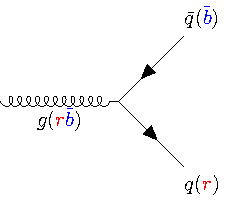
\includegraphics[width=0.25\textwidth]{SM/gqq.pdf}}
    \quad
    \subfloat[]{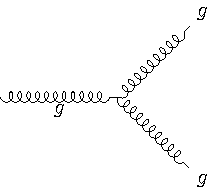
\includegraphics[width=0.25\textwidth]{SM/ggg.pdf}}
    \quad
    \subfloat[]{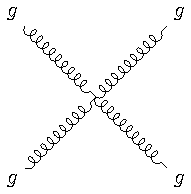
\includegraphics[width=0.25\textwidth]{SM/gggg.pdf}}
    \caption{Vertices allowed in QCD: (a) quark-gluon coupling, (b) three-point gluon self-coupling, and (c) four-point gluon self-coupling. The colour charge is shown in the quark-gluon vertex to depict an example of the interaction.}
    \label{figSM:QCDfey}
    \end{center}
\end{figure}

This theory has two important characteristics: asymptotic freedom and confinement~\cite{PhysRevLett.30.1346,PhysRevLett.30.1343}. Asymptotic freedom refers to the fact that at very high energies (in momentum transfer), or short distances, quarks and gluons interact weakly with each other allowing predictions to be obtained using perturbation theory. Confinement is the name given to the impossibility of directly observing quarks, which are only confined in hadrons, which are colourless composite states\footnote{Colour singlets are quantum states that are invariant under all eight generators of $SU(3)$ and therefore carry vanishing values of all colour conserved charges.}.\\

The idea is that for long distances, the strong coupling becomes larger, so when the distance between two quarks increases, the energy of the gluon field becomes larger, up to the point where a quark/anti-quark pair is created from the vacuum and thus a new hadron is formed. These characteristics arise from the non-abelian nature of the symmetry, which prompt the coupling to decrease with the energy of the interaction.

\subsubsection{Running coupling}

To understand the fact that the couplings can vary with the energy, the topics of \acrshort{QFT} renormalisation and regularisation have to be introduced. The quantity known as the matrix amplitude has to be computed for the prediction of physical quantities of a given process. Observables are proportional to the square sum of the amplitude of every possible Feynman diagram that yields the same initial and final particles of the process. However, the computation of diagrams with loops leads to the integration of all possible four-momentum of the virtual particles involved, which are divergent. Nevertheless, these divergences can be isolated with regularisation techniques, which render them finite by introducing a parameter $\Lambda$ such that for a given value of the parameter the divergence is recovered. This allows the computation of any quantity in terms of the \textit{bare} quantities that appear in the Lagrangian, such as masses or couplings, while incorporating the regularization parameter. The other key point is the renormalisation which arise from the idea that the physical quantities measured in experiments (masses or couplings) are different from the bare quantities (masses or couplings that appear in the lagrangian). Therefore, one has the freedom to apply renormalisation conditions, which cause the expressions to depend only on the physical quantities if the theory is renormalisable, and remove the divergent sources.\\

As an example, to compute the gluon two-point function, an infinite sum of loop contributions is needed,
\begin{align}
\begin{gathered}
    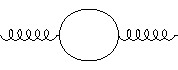
\includegraphics[width=0.25\textwidth]{SM/gluonSEA.pdf}
\end{gathered}&=\begin{gathered}
\includegraphics[width=0.25\textwidth]{SM/gluonSEB.pdf}
\end{gathered}+\begin{gathered}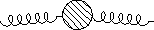
\includegraphics[width=0.25\textwidth]{SM/gluonSEC.pdf}
\end{gathered}+...
\end{align}

Focusing on the one loop contribution, the result is obtained at first order from three different diagrams,


\begin{align}
    \begin{gathered}
        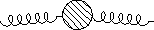
\includegraphics[width=0.25\textwidth]{SM/gluonSEC.pdf}
    \end{gathered}&=\begin{gathered}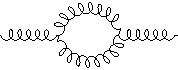
\includegraphics[width=0.2\textwidth]{SM/gluonLoopC.pdf}
    \end{gathered}+\begin{gathered}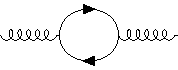
\includegraphics[width=0.2\textwidth]{SM/gluonLoopA.pdf}
    \end{gathered}+\begin{gathered}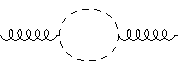
\includegraphics[width=0.2\textwidth]{SM/gluonLoopB.pdf}
    \end{gathered}+ ...
    \end{align}


which are the loop involving gluons, quarks and a third one with a new propagator, the ghost. This last propagator is a regularisation artifact to compensate unphysical degrees of freedom\footnote{There are other methods to avoid the unphysical degrees of freedom, like choosing a physical gauge in the axial direction.}. Focusing on the gluon loop contribution,

\begin{equation}
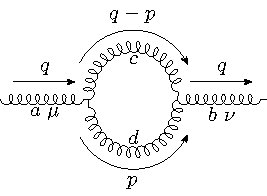
\includegraphics[width=0.25\textwidth]{SM/gluonLoopD.pdf}
\end{equation}

a badly divergent integral appears in its computation with Feynman rules,  

\begin{align}
    \begin{split} 
        \frac{1}{2}g_s^2f^{acd}f^{bcd}\int\frac{d^4p}{(2\pi)^4} \frac{1}{(q-p)^2+i\epsilon}\frac{1}{p^2+i\epsilon}&\qty[g^{\mu\alpha}(p-2q)^\beta+g^{\alpha\beta}(q-2p)^\mu+g^{\beta\mu}(p+q)^\alpha]\\
       &\qty[\delta_\alpha^\nu(p-2q)_\beta+g_{\alpha\beta}(q-2p)^\nu+\delta_\beta^\nu(p+q)_\alpha],
       \label{ipi}
    \end{split}
    \end{align}

which can be worked around with a regularisation parameter $\mu$,

\begin{equation*}
    \int \frac{d^4p}{(2\pi)^4}\to \int \frac{d^Dp}{(2\pi)^D}\mu^{2\varepsilon},
\end{equation*}\\

with $D=4-2\varepsilon$ where the limit $\varepsilon\to 0$ recovers the original expression. After the computation of all main contributions, the divergent term can be summarised as

\begin{equation}
    \frac{g_s^2}{24\pi}\qty[11n_c-2 n_f]\frac{1}{\epsilon}+\mathcal{O}(g_s^4),
\end{equation}

with $n_c$ the number of colours, $n_f$ the number of quark flavours and $\varepsilon\to 0$ the condition to recover the original divergence. Hence, the bare coupling constant can be rewritten to account for this divergence, thus completing the regularisation process for the gluon self-energy.\\

The final strong coupling constant is commonly given by 

\begin{equation}
    \label{Theory_eq:runningcoupling}
    \alpha_s(Q^2) = \frac{12\pi}{(11n_c - 2 n_f)\log \frac{Q^2}{\Lambda^2_\text{QCD}}},
\end{equation}

which depends on the energy scale $Q$ at which is evaluated and $\Lambda_\text{QCD}$ being the infrared cutoff scale that sets the validity of the perturbative regime of \acrshort{QCD}. As $n_c=3$, for $n_f$<16 the coupling constant decreases with the energy scale, which is the key feature of \acrshort{QCD} that causes asymptotic freedom and confinement.

\subsection{Electroweak theory}

The quantum field theory that describes both the electromagnetic and weak interactions is called \textit{\acrlong{EW}} theory. The theory is based on the $SU(2)_L\otimes U(1)_Y$ symmetry group\footnote{$L$ refers to the left-handed chirality and $Y$ to the weak hypercharge}, which is a product that yields a non-abelian group, like $SU(3)_C$. The resulting group is chiral as it acts differently on left-handed and right-handed particles, specifically from $SU(2)_L$ acting only on left-handed particles. It spawns four mediators, corresponding to the number of generators.\\

The symmetry spontaneously breaks down through \textit{symmetry breaking} giving rise to the electromagnetic interaction,
mediated by the photon, and to the weak interaction, mediated by the $Z$ and $W^\pm$ bosons.
This process is described by the \textit{\acrlongpl{EWSB}}~(\acrshort{EWSB}), which occurs at $\sim$100~GeV, defined as the \acrshort{EW} energy scale, and after which only the $U(1)_Q$ symmetry is unbroken. The process of the \acrshort{EWSB} and the resulting effects are described in
more detail in Section~\ref{subsec:SSB}.\\

The interactions for the \acrshort{EW} sector can be obtained following the procedure described in general in Section~\ref{subsec:SMinteractions}. First, only left-handed fermion fields interact via the weak
interaction\footnote{As a consequence, parity can be violated in weak interactions~\cite{Lee,Wu}.},
transforming as doublets under $SU(2)_L$, whereas right-handed fermion fields do not interact weakly and thus transform as singlets,

\begin{equation}
\begin{split}
    \psi_L^i &= \begin{pmatrix}\ell^i_L\\ \nu^i_L \end{pmatrix}, \begin{pmatrix} u^i_L \\ d^i_L \end{pmatrix}\\
    \psi_R^i &= \ell^i_R, u^i_R, d^i_R
\end{split}
\end{equation}

with $i$ corresponding to the number of the generation. Fields labelled with $L$ and $R$ are left- and right-handed fields that are defined through the chirality operators $P_L$ and $P_R$, projecting a generic field into only its left- and right-handed components, respectively,

\begin{equation}
    \begin{split}
        \psi_L = P_L\psi = \frac{1}{2}(1-\gamma_5)\psi\\
        \psi_R = P_R\psi = \frac{1}{2}(1+\gamma_5)\psi
    \end{split}
\end{equation}

$\gamma_5$ is defined from the Dirac matrices $\gamma_5\equiv i\gamma^0\gamma^1\gamma^2\gamma^3$. Notice that there are no right-handed fields associated to the neutrinos. This convention exists to avoid the prediction of right-handed neutrinos, which would not interact with any of the forces described in the \acrshort{SMlabel}.\\

The $SU(2)_L$ group consists of three generators $\hat{T}_i$, which can be written as $\hat{T}_i=\sigma_i/2$ where $\sigma_i$ denotes the Pauli matrices. Also, the quantum number associated to the symmetry group is the weak isospin, $T$.
On the other hand, the $U(1)_Y$ group introduces the weak hypercharge quantum number, $Y$. After \acrshort{EWSB},
the Gell-Mann-Nishijima equation relates $Y$ to the third component of the weak isospin operator, $T_3$, and the electric charge $Q$ as

\begin{equation}
Q = Y+T_3.
\end{equation}

Regarding the \acrshort{EW} Lagrangian, four gauge fields need to be introduced to achieve invariance under $SU(2)_L\otimes U(1)_Y$: $W_{\mu\nu}^i$ ($i$=1,2,3) from $SU(2)_L$, and $B_\mu$ from $U(1)_Y$. The resulting Lagrangian is

\begin{equation}
\label{Theory_eq:EWlagrangian}
\begin{split}
    \mathcal{L}_{EW}&=i\sum_{f=l,q}\bar{f}(\gamma^\mu D_\mu)f - \frac{1}{4}W_{\mu\nu}^iW^{i\ \mu\nu} - \frac{1}{4}B_{\mu\nu}B^{\mu\nu}\\
    D_{\mu \ } &\equiv \partial_\mu - ig\frac{\sigma}{2}W_\mu^i-ig'YB_\mu \\
    W_{\mu\nu}^i &\equiv \partial_\mu W_\nu^i - \partial_\nu W_\mu^i +g\epsilon^{ijk}W_\mu^j W_\nu^k\\
    B_{\mu\nu}&\equiv\partial_\mu B_\nu - \partial_\nu B_\mu,
    \end{split}
\end{equation}

with $\epsilon^{ijk}$ being the Levi-Civita symbol, an antisymmetric tensor defined as $\epsilon^{ijk}\epsilon_{imn}=\delta^j_m\delta^k_n-\delta^j_n\delta^m_k$ with $i,j,k,l,m,n\in[1,2,3]$. Also, the $W_{\mu\nu}^i$ and $B_{\mu\nu}$ field tensors are defined to introduce the additional kinetic terms to the Lagrangian. The former contains a quadratic piece, due to the non-abelian nature of $SU(2)_L$, hence the full Lagrangian contains cubic and quartic self-interactions, as for the gluons in QCD. In contrast, the coupling constant $g$ increases rapidly with the energy scale. As previously metioned, mass terms for the gauge boson would break the gauge invariance. In this case, terms for the fermion masses would also break the symmetry as they would mix left- and right-handed fields, which transform differently under $SU(2)_L$.\\

When adding all the interactions described, the SM Lagrangian for all the fermions before \acrshort{EWSB} becomes

\begin{equation}
    \label{Theory_eq:SMbeforeEWSB}
    \begin{split}
    \mathcal{L}_{SM} &= \sum_f\sum_{\psi=L,e_R,Q_L,u_R,d_R} i\bar{\psi}^f\gamma^\mu D_\mu \psi^f\\
    &- \frac{1}{4}G^a_{\mu\nu}G^{a\_\mu\nu} - \frac{1}{4}W^i_{\mu\nu}W^{i\_\mu\nu} - \frac{1}{4}B_{\mu\nu}B^{\mu\nu}\\
    D_\mu &= \partial_\mu - i g_s T^a G^a_\mu - i g \frac{\sigma^i}{2}W_\mu^i - ig'YB_\mu.
    \end{split}
\end{equation}

\subsection{Spontaneous symmetry breaking and the Higgs mechanism}
\label{subsec:SSB}
The model described so far cannot reproduce the experimental observations; first, the different fermions and the weak force mediators have mass, and secondly, the $SU(2)_L\times U(1)_Y$ symmetry is not preserved in nature.\\

Even if the \acrshort{EW} gauge bosons were allowed to have mass, the theory would lack renormalisability and violate unitarity. Renormalisation is a collection of techniques that allows for the computation of measurable observables in \acrshort{QFT}, managing the various sources of infinities within the theory, such as those from self-interactions.
Unitarity is needed more in general in quantum mechanics to ensure proper time-evolution predictions of a quantum state. The longitudinal component of the massive boson is the cause of the problem,
as in a boosted frame where the four-momentum $p^\mu=(p^0,0,0,|\textbf{p}|)$, the parallel polarisation component of a massive boson, given by $\epsilon_\mu=(|\textbf{p}|/m,0,0,p^0)$, grows indefinitely with the energy of the system.
When computing the cross-section of the corresponding boson scattering the value indefinitely grows breaking the mentioned unitarity.
When computed explicitly for the $W^\pm$ bosons, the energy scale where this occurs is around the TeV scale, which highlights a fundamental problem in the theory's ability to describe this scale.\\

The solution is provided by the \acrshort{EWSB} and the Higgs-Englert-Brout mechanism, discussed next, after showing the spontaneous
symmetry breaking process for a simple gauge theory.

\subsubsection{Breaking a symmetry}

Spontaneous symmetry breaking is a phenomenon where a symmetry of the theory is unstable and the vacuum, or fundamental state, is degenerate.
In the process of breaking a symmetry, new interactions appear and a field obtains a non-zero vacuum expectation value.\\

The topic is broad as there are many symmetries and representations that can be potentially broken with this mechanism. To illustrate the method for the \acrshort{SMlabel},
let's consider a system with a scalar field $\phi$, a gauge field $A_\mu$, and the following Lagrangian with a gauge symmetry,

\begin{equation}
    \begin{split}
    \mathcal{L}_{\ \ }&=(D^\mu\phi)^\dag D_\mu\phi - V(\phi) - \frac{1}{4}F_{\mu\nu}F^{\mu\nu}\\
    D_{\mu \ } &\equiv \partial_\mu - igA_\mu\\
    F_{\mu\nu}&\equiv\partial_\mu A_\nu - \partial_\nu A_\mu,
    \end{split}
\end{equation}

with a general potential $V(\phi)$ given by

\begin{equation}
    V(\phi) = \frac{1}{2}\mu^2\phi^\dag\phi + \frac{1}{4}\lambda(\phi^\dag\phi)^2,
\end{equation}

with the real parameters $\mu^2$ and $\lambda$ relating to the mass term and the strength of the self-interaction, respectively.
There are two sensible ranges for these parameters, depicted in Figure~\ref{figSM:higgspotential}, the first one is the case $\lambda>0,\mu^2>0$,
similar to the previous theories, with only one solution in the minimisation.
The second one is for $\lambda>0$ and $\mu^2<0$, where the $\mu^2\phi^\dag\phi$ term cannot be understood as a mass term and
the solution $\phi=0$ is a local maximum, physically unstable. The minimum of the potential is degenerate and identified by the complex
plane circle, $\phi^\dag\phi=v^2/2$ with $v^2\equiv-\mu^2/\lambda$ and $\phi = v e^{-i\theta}$.\\

\begin{figure}[htbp]
    \RawFloats
    \begin{center}
    \subfloat[]{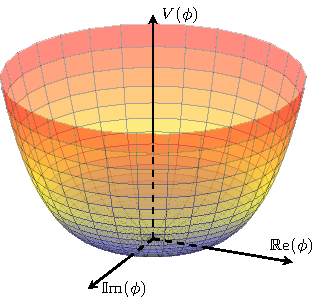
\includegraphics[width=0.4\textwidth]{SM/HiggspotentialA.pdf}}
    \qquad
    \subfloat[]{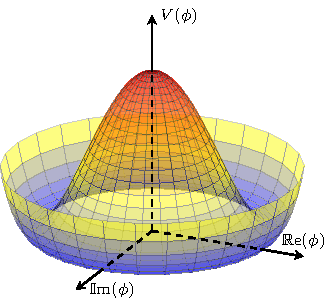
\includegraphics[width=0.4\textwidth]{SM/HiggspotentialB.pdf}}
    \caption{Shape of the potential $V(\phi)$ for $\lambda>0$ and (a) $\mu^2>0$ or (b) $\mu^2<0$.
    }
    \label{figSM:higgspotential}
    \end{center}
\end{figure}

The symmetry is broken spontaneously when the system chooses the fundamental state. In the case of $\phi=0$ the \textit{\acrlongpl{VEV}}~(\acrshort{VEV})
of $\phi$ is set to

\begin{equation}
    \expval{\phi}{0} = \frac{v}{\sqrt{2}}.
\end{equation}

Next, let's suppose the following change of variables to center the new fundamental state

\begin{equation}
    \phi(x)=\left( \frac{v+\eta(x)}{\sqrt{2}} \right) e^{i\zeta(x)/v}.
\end{equation}

In this case the Lagrangian can be expressed as

\begin{equation}
\begin{split}
\mathcal{L} &= \frac{1}{2}(\partial_\mu\eta)^2 + \frac{1}{2}(\partial_\mu\zeta)^2 - \frac{1}{4}F_{\mu\nu}F^{\mu\nu}\\
&+\mu^2\eta^2 + \frac{1}{2}g^2v^2A_\mu A^\mu - gv A\mu \partial^\mu\zeta +\ \text{interactions},
\end{split}
\end{equation}

which now contains the $\eta$ and $\zeta$ fields, additional to the gauge $A_\mu$. Also, square terms appear for $\eta$ and $A_\mu$,
which can be identified as mass terms, $\frac{m_\eta}{2}\eta^2$ and $\frac{m_A}{2}A_\mu A^\mu$,
resulting in $m_\eta=\sqrt{-2\mu^2}$ and $m_A=gv$. $\zeta(x)$ is massless and a particular resulting type of field named
\textit{Goldstone boson}, which the \textit{Goldstone theorem} predicts~\cite{Goldstone:1962es}.
The theorem states that a massless boson appears for every symmetry that the \acrshort{VEV} spontaneously breaks.
In this abelian case, the \acrshort{VEV} is not invariant under the $U(1)$ transformation.
$\zeta(x)$ does not appear explicitly in the potential, therefore it can take any value without affecting the energy of the system,
which is not very physical. In addition, it appears in a strange mixing term with $A_\mu$, $-gvA_\mu\partial^\mu\zeta$.\\

A way to remove the unphysical term is to choose the gauge

\begin{equation}
\begin{split}
    &\phi\rightarrow\phi'=e^{-i\zeta/v}\phi \\
    &A_\mu\rightarrow A'_\mu = A_\mu-\frac{1}{gv}\partial_\mu\zeta.
\end{split}
\end{equation}
together with the previous change of variable for $\phi$. Essentially the gauge freedom of the Lagrangian is being used to remove $\zeta$,
which becomes the longitudinal component of the transformed gauge boson $A_\mu$.
The gauge chosen is the so-called \textit{unitary gauge}, which makes the physical content of the Lagrangian explicit\footnote{The ghost gluons in the context of regularisation also remove the problematic unphysical degrees of freedom.}.\\

In summary, this process of acquiring mass by means of absorbing a Goldstone boson is known as the \textit{Higgs mechanism}.

\subsubsection{The Higgs-Englert-Brout Mechanism in the Electroweak Sector}

The Higgs-Englert-Brout mechanism~\cite{Higgs1,Higgs2,Englert} solves the contradictions found between massive particles and
the requirement of gauge invariance. The mechanism is based on a spontaneous symmetry breaking of the $SU(2)_L\otimes U(1)_Y$ to $U(1)_{EM}$,
giving mass to the different particles involved in the \acrshort{EW} interactions apart from the photon.\\

A similar procedure can be applied to the EW Lagrangian derived in Equation~\ref{Theory_eq:SMbeforeEWSB},
first by introducing an isospin doublet ($Y$=+1/2) of complex scalar fields $\Phi$, the Higgs field, defined as

\begin{equation}
    \Phi\equiv
    \begin{pmatrix} \phi^+ \\ \phi^0 \end{pmatrix}
    =\frac{1}{\sqrt{2}}
    \begin{pmatrix} \phi_1 + i\phi_2 \\ \phi_3 + i\phi_4 \end{pmatrix},
\end{equation}

where $\phi^+$ corresponds to an electrically charged field ($T_3$=+1/2) and $\phi^0$ to a neutral one ($T_3$=-1/2).
This field transforms under $SU(2)_L$ and the Lagrangian, the Higgs Lagrangian, can be written as

\begin{equation}
    \mathcal{L}_\Phi = (D_\mu\Phi)^\dag(D^\mu\Phi)-V(\Phi),
\end{equation}

with the same covariant derivative as in Equation~\ref{Theory_eq:SMbeforeEWSB} and the Higgs potential given by

\begin{equation}
    V(\Phi) = \mu^2\Phi^\dag\Phi+\lambda(\Phi^\dag\Phi)^2,
\end{equation}

whose shape depends on the parameters $\mu^2$ and $\lambda$. As seen before, choosing the case where $\lambda>0$ and $\mu^2<0$,
the potential at $\Phi=0$ is unstable, and a continuous collection of possible minimum values appear defined by the circle

\begin{equation}
    \Phi^\dag\Phi=\frac{1}{2}\frac{-\mu^2}{\lambda}\equiv\frac{1}{2}v^2.
\end{equation}

The symmetry is spontaneously broken with the choice of a new vacuum state,

\begin{equation}
    \expval{\Phi}{0} =\frac{1}{\sqrt{2}}\begin{pmatrix}
    0\\v
    \end{pmatrix}.
\end{equation}

This vacuum is not invariant to either of the $SU(2)_L$ or the $U(1)$ transformations. However, the $Q=T_3+Y$ transformation is not affected:

\begin{equation}
    Q\expval{\Phi}{0} = \frac{1}{2\sqrt{2}}\sigma_3\begin{pmatrix}0\\v\end{pmatrix}+\frac{1}{2\sqrt{2}}Y\begin{pmatrix}0\\v\end{pmatrix} = \frac{1}{2\sqrt{2}}\left[ 
    \begin{pmatrix} 0 \\ -v  \end{pmatrix} +
    \begin{pmatrix} 0 \\ v  \end{pmatrix}\right] = \begin{pmatrix}
    0\\0
    \end{pmatrix}.
\end{equation}

The field is rewritten in the unitary gauge, which automatically removes the extra non-physical Goldstone bosons,

\begin{equation}
    \Phi(x) = \frac{1}{\sqrt{2}}\begin{pmatrix}
    0 \\ v+H(x)
    \end{pmatrix},
\end{equation}

where $H(x)$ is centered around the vacuum state. With this change the Higgs potential becomes

\begin{equation}
    V(\Phi) =\frac{1}{4}\lambda v^2 H^2 + \frac{1}{4} \lambda v H^3 + \frac{1}{16} \lambda H^4,
\end{equation}

spawning the Higgs boson mass in the quadratic $H$ term, $m_H^2=\lambda v^2/2 = -\mu^2/2$.
The cubic and quartic terms correspond to the three- and four-point Higgs boson self-interactions.\\

The \acrshort{EWSB} generates new interactions and mass terms for the different particles involved in the \acrshort{EW} interactions.
Gluons are not affected as the scalar field is a doublet and does not transform under $SU(3)$. The effects on the boson and fermion sectors of the \acrshort{SMlabel} are discussed individually in the following. 

\subsubsection{Boson sector}

The gauge boson masses arise from the covariant derivative, $(D_\mu\Phi)^\dag(D^\mu\Phi)$, which includes the gauge fields. The expression for $\mathcal{L}_{mass}$ is found expanding $(D_\mu\Phi)^\dag(D^\mu\Phi)$ and focusing on the $V_\mu V^\mu$ term,

\begin{equation}
\label{Theory_eq:Lgaugemass}
\mathcal{L}_{mass} = \frac{v^2}{8}
V_\mu
\begin{pmatrix} \begin{matrix} g^2 & 0 \\ 0 & g^2 \end{matrix} & 0_{2\times2} \\ 0_{2\times2} & \begin{matrix} g^2 & -gg' \\ -gg' & g'^2 \end{matrix}
\end{pmatrix} V^\mu ,
\end{equation}

with $V_\mu = \begin{pmatrix} W_\mu^1 & W_\mu^2 & W_\mu^3 & B_\mu
\end{pmatrix}$. After diagonalising the matrix the following eigenvectors are found:

\begin{equation}
\begin{split}
    A_\mu &\equiv \sin\theta_W W_\mu^3 + \cos\theta_WB_\mu \\
    Z_\mu &\equiv \cos\theta_W W_\mu^3 - \sin\theta_WB_\mu,
\end{split}
\end{equation}

where the Weinberg angle, or weak mixing angle, is defined by $\tan\theta_W\equiv g'/g$. The eigenvalues are the square of the masses of the different bosons, which are zero and $v^2(g^2+g'^2)/8$ for the $A_\mu$ and $Z_\mu$ fields, respectively. In contrast, $W_\mu^1$ and $W_\mu^2$ are well-defined mass states but not charge states. This is due to $T_1$ and $T_2$ being not diagonal, connecting the different states of $T_3$ (hence of $Q$). The operator $T_\pm=T_1\mp iT_2$ can be defined, which increases or decreases one unit of $T_3$ (hence of $Q$). In addition, the fields can be redefined as

\begin{equation}
    W_\mu^\pm = \frac{1}{\sqrt{2}}(W_\mu^1\mp i W_\mu^2).
\end{equation}

In summary the Lagrangian in Equation~\ref{Theory_eq:Lgaugemass} can now be written as

\begin{equation}
    \mathcal{L}_{mass} = \frac{g^2v^2}{4}W_\mu^+W^{- \mu} - \frac{v^2}{8}(g^2+g'^2)Z_\mu Z^\mu,
\end{equation}

where the mass terms of the different bosons can be identified,

\begin{equation}
\begin{split}
    &m_A = 0\\
    &m_Z = \frac{v}{2}\sqrt{g^2+g'^2}\\
    &m_W = \frac{vg}{2} = m_Z \cos\theta_W.
\end{split}
\end{equation}

Note that the remaining symmetry after breaking $SU(2)_L\otimes U(1)_L$ is $U(1)_{EM}$. The associated $A_\mu$ field is massless, the photon, which is a combination of the $W_\mu^3$ and $B_\mu$ fields. The associated quantum number, the electric charge, has been defined previously in the chapter, $Q = T_3-Y$.\\

Concerning the interactions, the covariant derivative can be expressed in terms of the new bosons as

\begin{equation}
    \partial_\mu - igW_\mu^3 = \partial_\mu - ig\sin\theta_W A_\mu - ig\cos\theta_W Z_\mu,
\end{equation}

where the electromagnetic coupling constant $e$ can be defined as $e=g\sin\theta_W$. In addition, the field tensors can be rewritten as

\begin{equation}
\begin{split}
    W_{\mu\nu}^3 &= \partial_\mu W_\nu^3 - \partial_\nu W_\mu^3 - ig(W_\mu^+W_\nu^- - W_\nu^+ W_\mu^-)\\
    &= \sin\theta_W F_{\mu\nu} + \cos\theta_W Z_{\mu\nu} - ig(W_\mu^+W_\nu^- - W_\nu^+ W_\mu^-)\\
    B_{\mu\nu} &= \cos\theta_W F_{\mu\nu} - \sin\theta_W Z_{\mu\nu},
\end{split}
\end{equation}

where the field strength tensors for the photons and the Z boson, $F_{\mu\nu}$ and $Z_{\mu\nu}$ are included.

\subsubsection{Fermion sector}%\vspace{-\baselineskip}

The procedure required to obtain the fermion masses is more complicated than for the gauge bosons. Instead of just expanding the kinematic term with the new Higgs field, Yukawa~\cite{yukawa} interactions that couple left- and right-handed fermions with the Higgs need to be introduced.\\

As mentioned previously, only $q_{\alpha L}^i$ and $l^i_L$ fields are $SU(2)_L$ doublets,

\begin{equation}
    \label{Theory_eq:SUdoublets}
    q_{\alpha L}^i=\begin{pmatrix} u^i_{\alpha L} \\ d^i_{\alpha L} \end{pmatrix},\ l_L^i = \begin{pmatrix} \nu^i_L \\ \ell^i_L \end{pmatrix}
\end{equation}

where the $i$ refers to the generation and $\alpha$ to the colour. It has already been pointed out that is not possible to construct a well defined $mf^\dag f$ term that transforms under the SM group, necessary for gauge invariance. The solution is provided by introducing Yukawa interactions between the fermion fields and the Higgs field $\Phi$, also a doublet under $SU(2)$,

\begin{equation}
\begin{split}
    &\mathcal{L}_{Yukawa} = -y^{ab}\bar{q}^a_{\alpha\ L}\Phi d^b_{\alpha\ R} - y'^{ab}\bar{q}^a_{\alpha\ L}\tilde{\Phi} u^b_{\alpha\ R}-y''^{ab}\bar{l}^a_{L}\Phi \ell^b_{R}+\ \text{h.c}\\
    %&-\epsilon^{ij}\Phi_i (q_{\alpha\ L})^a_j y^{ab} (\bar{d}_{\alpha\ L})^b_{\alpha}
    %-\epsilon^{ij}\Phi_i (q_{\alpha\ L})^a_j y^{ab} (\bar{d}_{\alpha\ L})^b_{\alpha}
\end{split}
\end{equation}

where y, y' and y'' are the Yukawa matrices, $3\times3$ matrices with one dimension for each generation. Also, $\tilde{\Phi}\equiv i\sigma_2\Phi^*$. Note that there is no second term for the leptons, as the SM does not contemplate the right handed neutrino, $\nu_R$. Also, this Lagrangian breaks explicitly the chiral symmetry but yields a singlet representation, safe for gauge invariance.\\

Next, writing the field $\Phi$ in terms of the unitary gauge as in the EWSB, $\phi^0(x)=v+H(x)$,

\begin{equation}
\begin{split}
    \mathcal{L}_{Yukawa} &= -\frac{1}{\sqrt{2}}(v+H)y^{ab}\bar{q}^a_{\alpha\ L} d^b_{\alpha\ R} - \frac{1}{\sqrt{2}}(v+H)y'^{ab}\bar{q}^a_{\alpha\ L}u^b_{\alpha\ R}\\
    &-\frac{1}{\sqrt{2}}(v+H)y''^{ab}\bar{l}^a_{L}\ell^b_{R}+\ \text{h.c}\\
    &=-\frac{1}{\sqrt{2}}(v+H)y^{ab} \bar{D}^a_\alpha D^b_\alpha - \frac{1}{\sqrt{2}}(v+H)y'^{ab}\bar{U}^a_\alpha U^b_\alpha\\
    &-\frac{1}{\sqrt{2}}(v+H)y''^{ab}\bar{L}^a L^b+\ \text{h.c}
\end{split}
\end{equation}

where the expression has been rearranged to define Dirac fields in spinor notation,

\begin{equation}
\label{Theory_eq:Diracmassspace}
    D_\alpha^a = \begin{pmatrix} d_\alpha^a \\ \bar{d}^{\dag a}_\alpha \end{pmatrix},\ 
    U_\alpha^a = \begin{pmatrix} u_\alpha^a \\ \bar{u}^{\dag a}_\alpha \end{pmatrix},\ 
    L_\alpha^a = \begin{pmatrix} \ell_\alpha^a \\ \bar{\ell}^{\dag a}_\alpha \end{pmatrix}
\end{equation}

After diagonalising the three Yukawa matrices, the eigenvalue terms are related to the masses, which can be identified for each generation as,

\begin{equation}
\begin{split}
m_{d^i} = y^{ii}v/\sqrt{2} \\ 
m_{u^i} = y'^{ii}v/\sqrt{2} \\
m_{\ell^i} = y''^{ii}v/\sqrt{2} \\
m_{\nu^i} = 0
\end{split}
\label{Theory_eq:yukawacouplings}
\end{equation}

There is a major consequence of the differences between the representation in the generator space (Equation~\ref{Theory_eq:SUdoublets}, $SU(2)_L$ doublets), and in mass space, after diagonalising the Yukawa matrices. $D^a_{\alpha}$ and $U^a_{\alpha}$ are rotated to diagonalise their corresponding Yukawa matrix, so affected by different transformations. However, the individual $d^a_{\alpha\ L}$ and $u^a_{\alpha\ L}$ fields are part of the same $SU(2)_L$ doublet.\\ 

The effect can be seen writing the $W^\pm$ interactions in the mass state representation of the fields which become off-diagonal,

\begin{equation}
    \frac{-g}{\sqrt{2}} \begin{pmatrix} \bar{u}_L & \bar{c}_L & \bar{t}_L \end{pmatrix} \gamma^\mu W_\mu^+ V_{CKM} \begin{pmatrix} d_L \\ s_L \\ b_L \end{pmatrix} +\ \text{h.c}
\end{equation}
\begin{equation}
\begin{pmatrix} d'_L \\ s'_L \\ b'_L \end{pmatrix} = V_{CKM}\begin{pmatrix} d_L \\ s_L \\ b_L \end{pmatrix} =\begin{pmatrix} V_{ud} & V_{us} & V_{ub} \\ V_{cd} & V_{cs} & V_{cb} \\ V_{td} & V_{ts} & V_{tb} \end{pmatrix} \begin{pmatrix} d_L \\ s_L \\ b_L \end{pmatrix}
\end{equation}

where the superscript ' denotes the mass representation and $V_{CKM}$ is the Cabibbo-Kobayashi-Maskawa matrix~\cite{Cabibbo,KobayaMaska}. This unitary matrix is the product of the transformations that diagonalise the y and y' Yukawa matrices, which encodes the mixing of the different generations of fields in charged-mediated weak interactions. This is known as flavour violation, where a weak interaction of a quark can result on changing its flavour. %\todo{feynman diagram?}
On the other side, leptons are represented with the same $SU(2)_L$ doublet, so any mixing of lepton generations is not present in the theory.\\

There is still another interesting feature that arises from the CKM matrix. The standard representation~\cite{Ling-Lie} of the matrix takes into account invariant phase rotations of the fields, leaving as free parameters three angles $\theta_{12}$, $\theta_{23}$ and $\theta_{13}$ (chosen to lie in the first quadrant so $\sin\theta,\cos\theta\geq0$), and a single complex phase $\delta$ that cannot be rotated to zero. The matrix reads,

\begin{equation}
\begin{split}
    V_{CKM} &= \begin{pmatrix} 1 & 0 & 0 \\ 0 & c_{23} & s_{23} \\ 0 & -s_{23} & c_{23} \end{pmatrix} \begin{pmatrix} c_{13} & 0 & s_{13}e^{-i\delta} \\ 0 & 1 & 0 \\ -s_{13}e^{i\delta} & 0 & c_{13} \end{pmatrix}
    \begin{pmatrix} c_{12} & s_{12} & 0 \\ -s_{12} & c_{12} & 0 \\ 0 & 0 & 1 \end{pmatrix} \\ 
    &= \begin{pmatrix} c_{12}c_{13} & s_{12}c_{13} & s_{13}e^{-i\delta} \\ -s_{12}c_{23}-c_{12}s_{23}s_{13}e^{i\delta} & c_{12}c_{23}-s_{12}s_{23}s_{13}e^{i\delta} & s_{23}c_{13} \\ s_{12}s_{23}-c_{12}c_{23}s_{13}e^{i\delta} & -c_{12}s_{23}-s_{12}c_{23}s_{13}e^{i\delta} & c_{23}c_{13} \end{pmatrix}
\end{split}
\end{equation}

where $s_{ij}=\sin\theta_{ij}$ and $c_{ij}=\cos\theta_{ij}$. The presence of the complex phase leads to different couplings for anti-matter, as the complex phase will switch sign, thus leading to matter/anti-matter asymmetry. This asymmetry in flavour-changing processes is the only source in the \acrshort{SMlabel} of \textit{CP} violation, or \textit{T} violation (from the time-reversal symmetry\footnote{The three symmetries are related as the combination, $CPT$ symmetry, which must always be respected in theory.}) however, as discussed in Section~\ref{subsec:openquestions}, fails to describe the current matter/anti-matter content of the universe. The CKM matrix is predicted and measured to be almost diagonal, with very small sources of CP violation, or $V_{ub}$ and $V_{td}$.\\

The current matrix as in 2022~\cite{pdg} reads, 
\begin{equation}
        V_{CKM}= \begin{pmatrix} 0.97401 \pm 0.00011 & 0.22650 \pm 0.00048 & 0.00361^{+0.00011}_{-0.00009} \\ 0.22636 \pm 0.00048 & 0.97320 \pm 0.00011 & 0.04053^{+0.00083}_{-0.00061} \\ 0.00854^{+0.00023}_{-0.00016} & 0.03978^{+0.00082}_{-0.00060} & 0.999172^{+0.000024}_{-0.000035} \end{pmatrix}
\end{equation}

\subsection{Flavour Changing Neutral Currents interactions}
\label{Theory_SMsubsec:FCNC}
\textit{Flavour Changing Neutral Currents} (FCNC) are the processes that involve the change of a fermion flavour through a neutral boson. In the electroweak sector, the neutral current interactions are mediated by the $Z$ boson. Contrary to the $W^\pm$ case, the interactions involving the $Z$ boson involve fields with the same associated Yukawa matrix, from the same spinors of the mass representation (Equation~\ref{Theory_eq:Diracmassspace}). Hence, no mixing matrix is spawned and thus no explicit FCNC appear in the \acrshort{SMlabel} Lagrangian.\\

The existence of charged flavour changing currents is allowed at tree level but their associated couplings are proportional to the off-diagonal elements of the CKM matrix, which are especially small for the interactions between the first and third generation leptons. However, FCNC processes can be obtained from consecutive flavour changing interactions in higher order diagrams. Figure~\ref{figSM:FCNCdiagrams} shows example FCNC processes involving the two types of first order Feynman diagrams, known as \textit{box} and \textit{penguin} diagrams.

\begin{figure}[htbp]
    \RawFloats
    \begin{center}
        \subfloat[]{\raisebox{0.45\height}{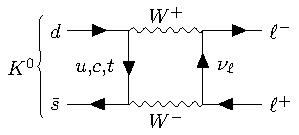
\includegraphics[width=0.48\textwidth]{SM/boxdiagram.pdf}}}
        \quad
        \subfloat[]{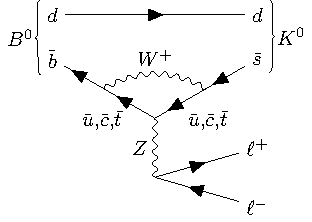
\includegraphics[width=0.48\textwidth]{SM/BKll.pdf}}
        \caption{
            Example first-order Feynman diagrams of a box diagram for the $K^0\to\ell^+\ell^-$ process (a) and of a penguin diagram for the $B^0\to K^0\ell^+\ell^-$ process (b). 
    }
    \label{figSM:FCNCdiagrams}
    \end{center}
\end{figure}

The high-order contributions are suppressed further by the Glashow, Iliopoulos and Maiani (GIM) mechanism~\cite{PhysRevD.2.1285}. In order to illustrate this mechanism, the example penguin diagram is discussed in the following. The diagram depicts a top FCNC decay that involves the $t\to b$ and $b\to c$ types of interactions, thus the interaction will be proportional to $V_{cb}^*V_{tb}$. Adding up the other two possible diagrams with $d$ and $s$ in the loop, 

\begin{equation}
    V_{cd}^*V_{td}+V_{cs}^*V_{ts}+V_{cb}^*V_{tb}
\end{equation}

which assumes that the quarks have the same mass. The value of this expression can be obtained from the CKM matrix. As the matrix is unitary ($V_{CKM}V_{CKM}^\dagger=V_{CKM}^\dagger V_{CKM}=\mathds{1}$), a total of 18 constraints appear, relating the different vertices: 

\begin{alignat*}{11}
    V_{ud}^2&+&V_{cd}^2&+&V_{td}^2&=1,   &\qquad V_{ud}^2&+&V_{us}^2&+&V_{ub}^2=1  \\
    V_{us}^2&+&V_{cs}^2&+&V_{ts}^2&=1,   &\qquad V_{cd}^2&+&V_{cs}^2&+&V_{cb}^2=1 \\
    V_{ub}^2&+&V_{cb}^2&+&V_{tb}^2&=1,   &\qquad V_{td}^2&+&V_{ts}^2&+&V_{tb}^2=1 \\
\end{alignat*}
\vspace{-1em}
\begin{alignat}{11}
    V_{ud}^*V_{us}&+&V_{cd}^*V_{cs}&+&V_{td}^*V_{ts}&=0,   &\qquad V_{ud}^*V_{cd}&+&V_{us}^*V_{cs}&+&V_{ub}^*V_{cb}&=0 \nonumber \\
    V_{ud}^*V_{ub}&+&V_{cd}^*V_{cb}&+&V_{td}^*V_{tb}&=0,   &\qquad V_{ud}^*V_{td}&+&V_{us}^*V_{ts}&+&V_{ub}^*V_{tb}&=0 \\ 
    V_{us}^*V_{ud}&+&V_{cs}^*V_{cd}&+&V_{ts}^*V_{td}&=0,   &\qquad V_{cd}^*V_{ud}&+&V_{cs}^*V_{us}&+&V_{cb}^*V_{ub}&=0 \nonumber\\
    V_{us}^*V_{ub}&+&V_{cs}^*V_{cb}&+&V_{ts}^*V_{tb}&=0,   &\qquad V_{cd}^*V_{td}&+&V_{cs}^*V_{ts}&+&V_{cb}^*V_{tb}&=0 \nonumber\\
    V_{ub}^*V_{ud}&+&V_{cb}^*V_{cd}&+&V_{tb}^*V_{td}&=0,   &\qquad V_{td}^*V_{ud}&+&V_{ts}^*V_{us}&+&V_{tb}^*V_{ub}&=0 \nonumber\\
    V_{ub}^*V_{us}&+&V_{cb}^*V_{cs}&+&V_{tb}^*V_{ts}&=0,   &\qquad V_{td}^*V_{cd}&+&V_{ts}^*V_{cs}&+&V_{tb}^*V_{cb}&=0 \nonumber
\end{alignat}

The equation is exactly one of the constraints and equals zero.  However, as the different quarks are not degenerate in mass, every term would be proportional to $1/m_q$ ($q$ being the quark inside the loop). This is the origin of the GIM mechanism and results in a non-zero but very suppressed contribution of FCNC in the \acrshort{SMlabel}. In addition, this suppression is larger for loops involving down-type quarks as their masses are more similar to each other than for the up-type quarks.

\section{Standard Model measurements and top physics}

Since the formulation of the \acrshort{SMlabel}, most experimental observations and measurements have been described successfully by the model. Throughout the years, predicted particles have been found and multiple precision measurements have tested its validity. However, there are theoretical and experimental issues that are not solved, leading to the conclusion that the \acrshort{SMlabel} is an effective theory and there is a more complete theory that can explain the whole range of observations.\\

In this section, a summary of the measurements of the \acrshort{SMlabel} is presented, focusing on processes involving the top quark and FCNC. Then, different main open questions of the \acrshort{SMlabel} are briefly reviewed.

\subsection{Experimental measurements}

Decades of experiments have performed measurements of parameters that define the \acrshort{SMlabel}. The \acrshort{SMlabel} can be summarised with nineteen parameters, which have been described in this chapter: nine fermion masses (six for quarks, three for leptons), the three gauge couplings ($g_S$, $g$ and $g'$), the Higgs vacuum expectation value ($v$), the Higgs mass, four parameters of the CKM matrix (three angles and a complex phase) and the \acrshort{QCD} CP-violating phase. There is no underlying relation between these parameters, only being set from experimental observations. With these parameters measured, theoretical predictions of observables can be tested with experimental data in order to explore new physics.\\

One typical observable in particle physics is the cross-section $\sigma$, the expected interaction rate between two interacting particles in terms of the effective surface area typically measured in \textit{pb} (picobarn, 1pb = 10$^{-40}$ m$^2$). The cross-section of a process depends on the interacting forces involved, as well as the energy and momentum of the interacting particles, which can be calculated from the S-matrix (scattering matrix) using relativistic mechanics. Feynman diagrams are a tool to translate a visual description of a process to a mathematical expression, the matrix amplitude, which is proportional to the probability of the specific process happening and is needed for the computation.\\

The decay width, $\Gamma$, can be computed in similar fashion to obtain another common observable, the Branching Ratio (BR). The BR of an unstable particle is the probability for it to decay into specific particles among all possible states. It is computed by dividing the $\Gamma$ of the specific process with respect to the sum of all the possible processes. Both $\sigma$ and $\Gamma$ are calculated from perturbation approximations, as the actual process is not the product of just one Feynman diagram, but all the possible interactions that lead to the same final state including loops, interferences and radiative corrections, refereed to as high order corrections. However, each particle interaction is proportional to the probability making higher order corrections become less important. Typically, \textit{leading-order} (LO) calculations use only the leading order terms from the perturbation expansion, while if complemented by higher order corrections are referred to next-to-leading-order (NLO) or next-to-NLO (NNLO) calculations.\\

Figure~\ref{figSM:xsecSM} shows a summary of a wide range of cross-section measurements by the \acrshort{ATLASlabel} Collaboration compared to the theoretical predictions, showing excellent agreement between data and theory. On the other side, the Higgs boson has been scrutinised since its discovery to characterise all its properties. Figure~\ref{figSM:xsecBRH} shows a summary of Higgs boson production cross-sections and branching ratios by the \acrshort{ATLASlabel} Collaboration, including the coupling strengths to other \acrshort{SMlabel} particles. It shows that the coupling is proportional to the mass of the resulting particle, as expected from the Higgs mechanism. As the Higgs couples with any particle that acquires mass through its field, it is an excellent candidate to study any other particle still to be discovered.\\

\begin{figure}[htbp]
    \RawFloats
    \begin{center}
    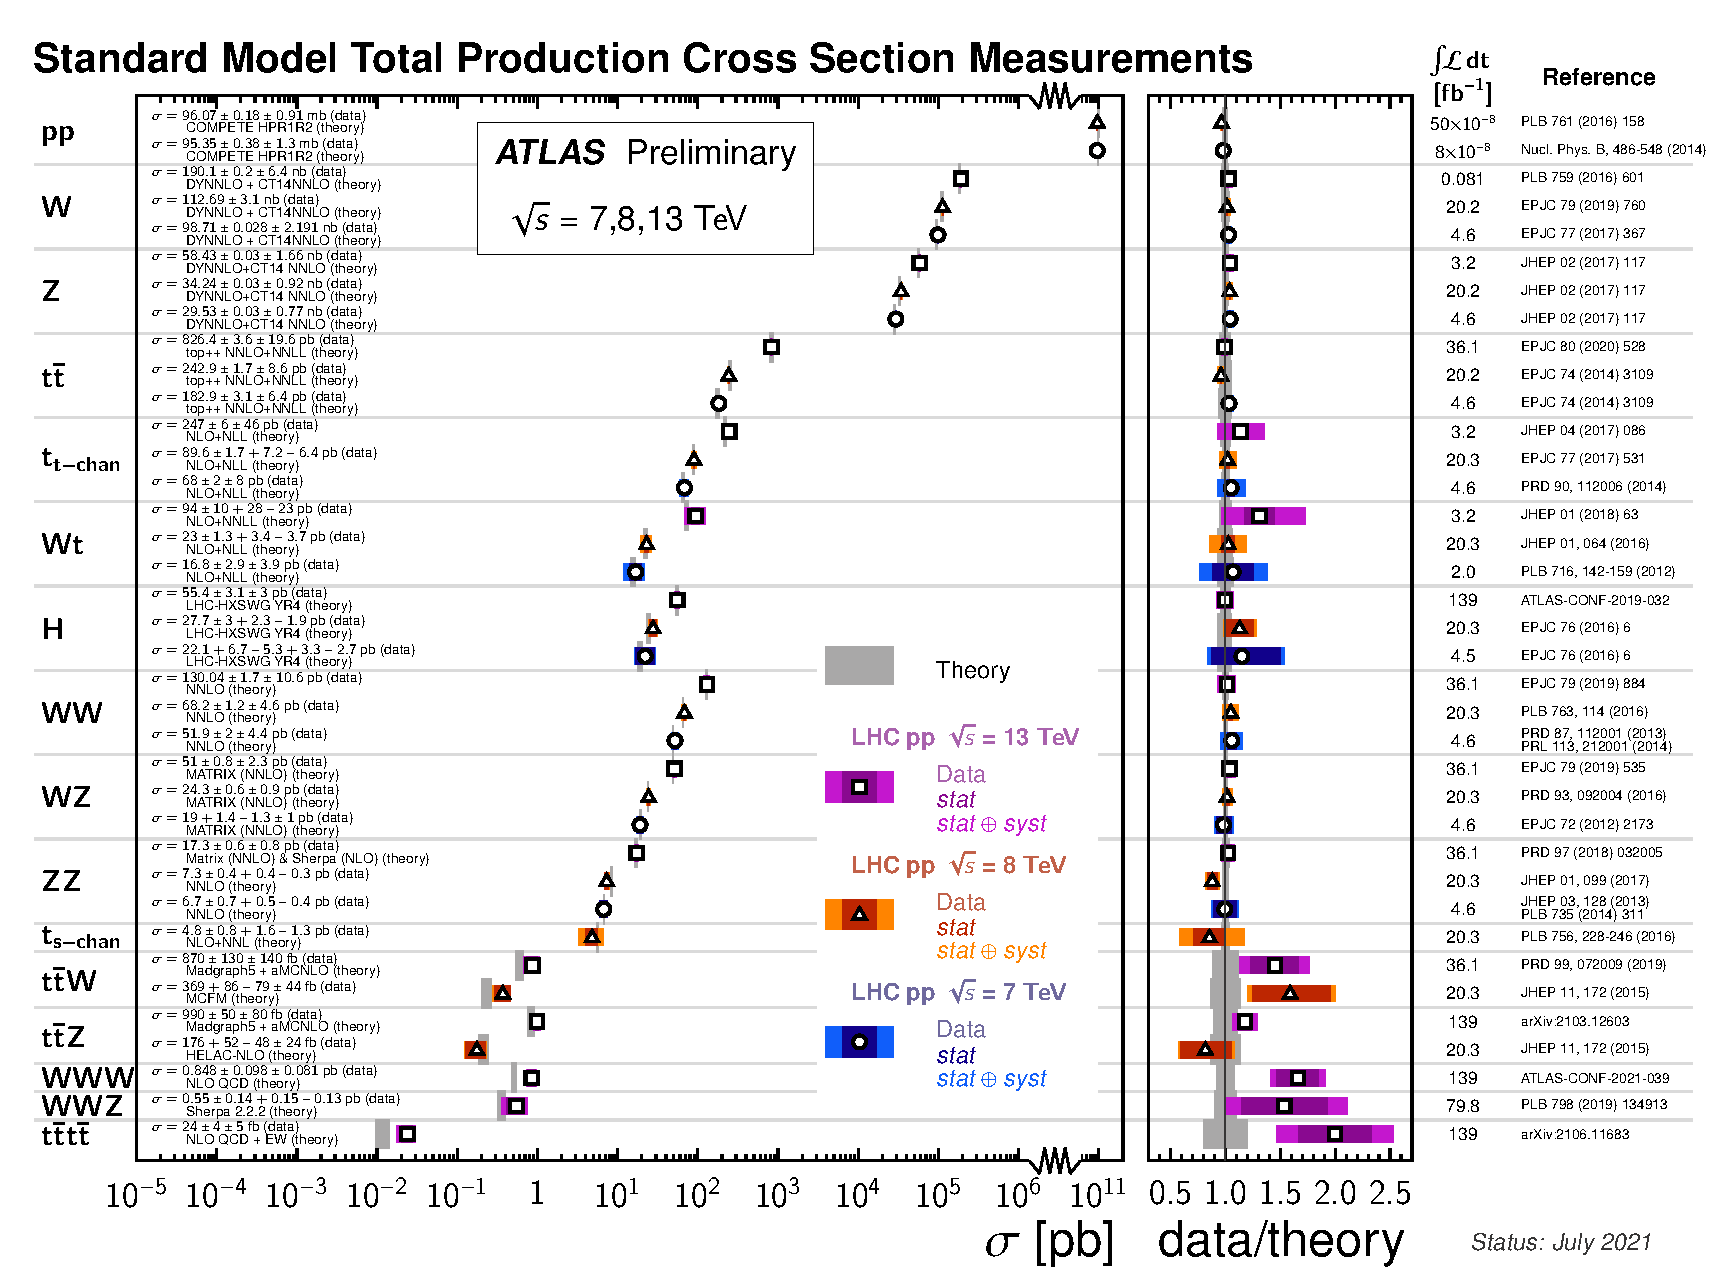
\includegraphics[width=1.0\textwidth]{SM/xsecSM.pdf}
    \caption{
        Summary of several \acrshort{SMlabel} total production cross-section measurements, corrected for branching fractions, compared to the corresponding theoretical predictions and ratio with respect to theory~\cite{ATLAS:2022djm}. 
    }
    \label{figSM:xsecSM}
    \end{center}
\end{figure}

\begin{figure}[htbp]
    \RawFloats
    \begin{center}
        \subfloat[]{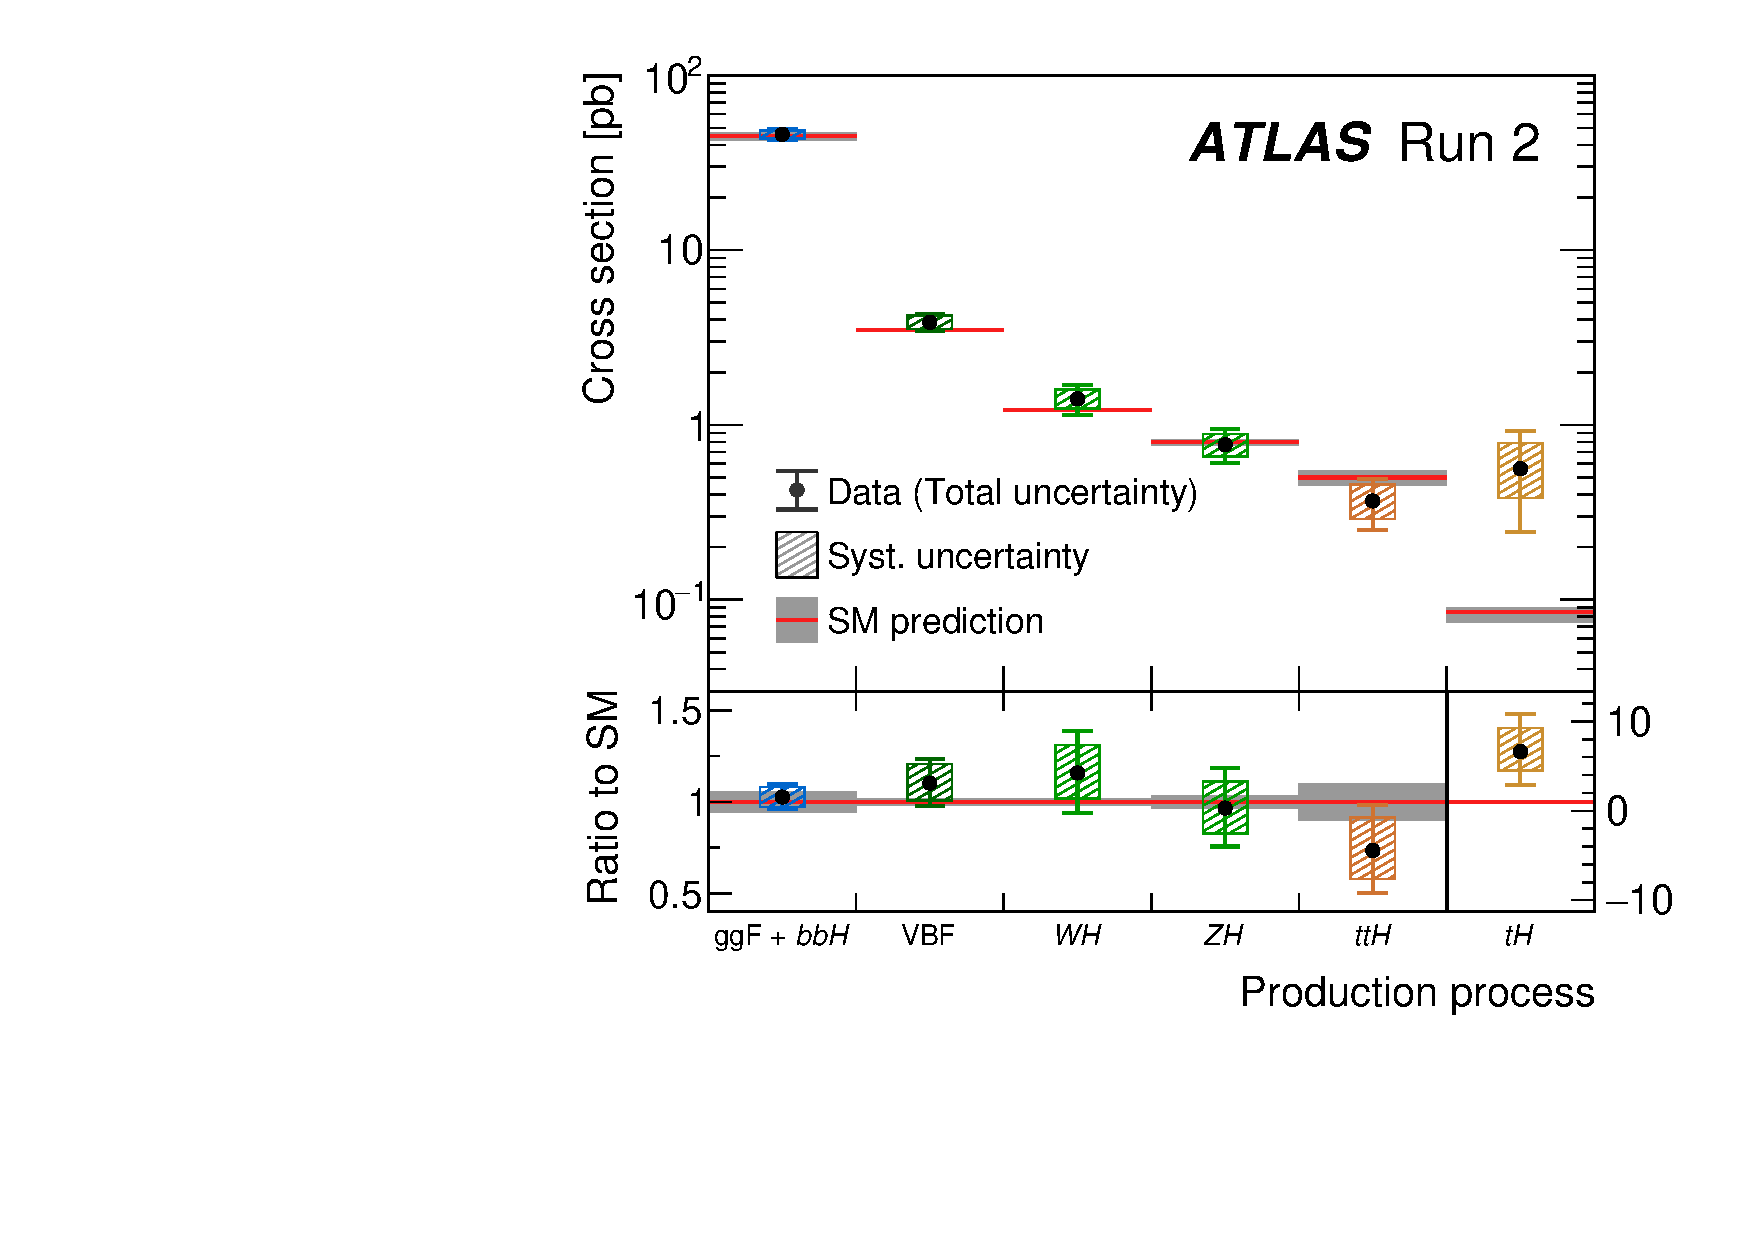
\includegraphics[width=0.48\textwidth]{SM/xsecH.pdf}}
        \quad
        \subfloat[]{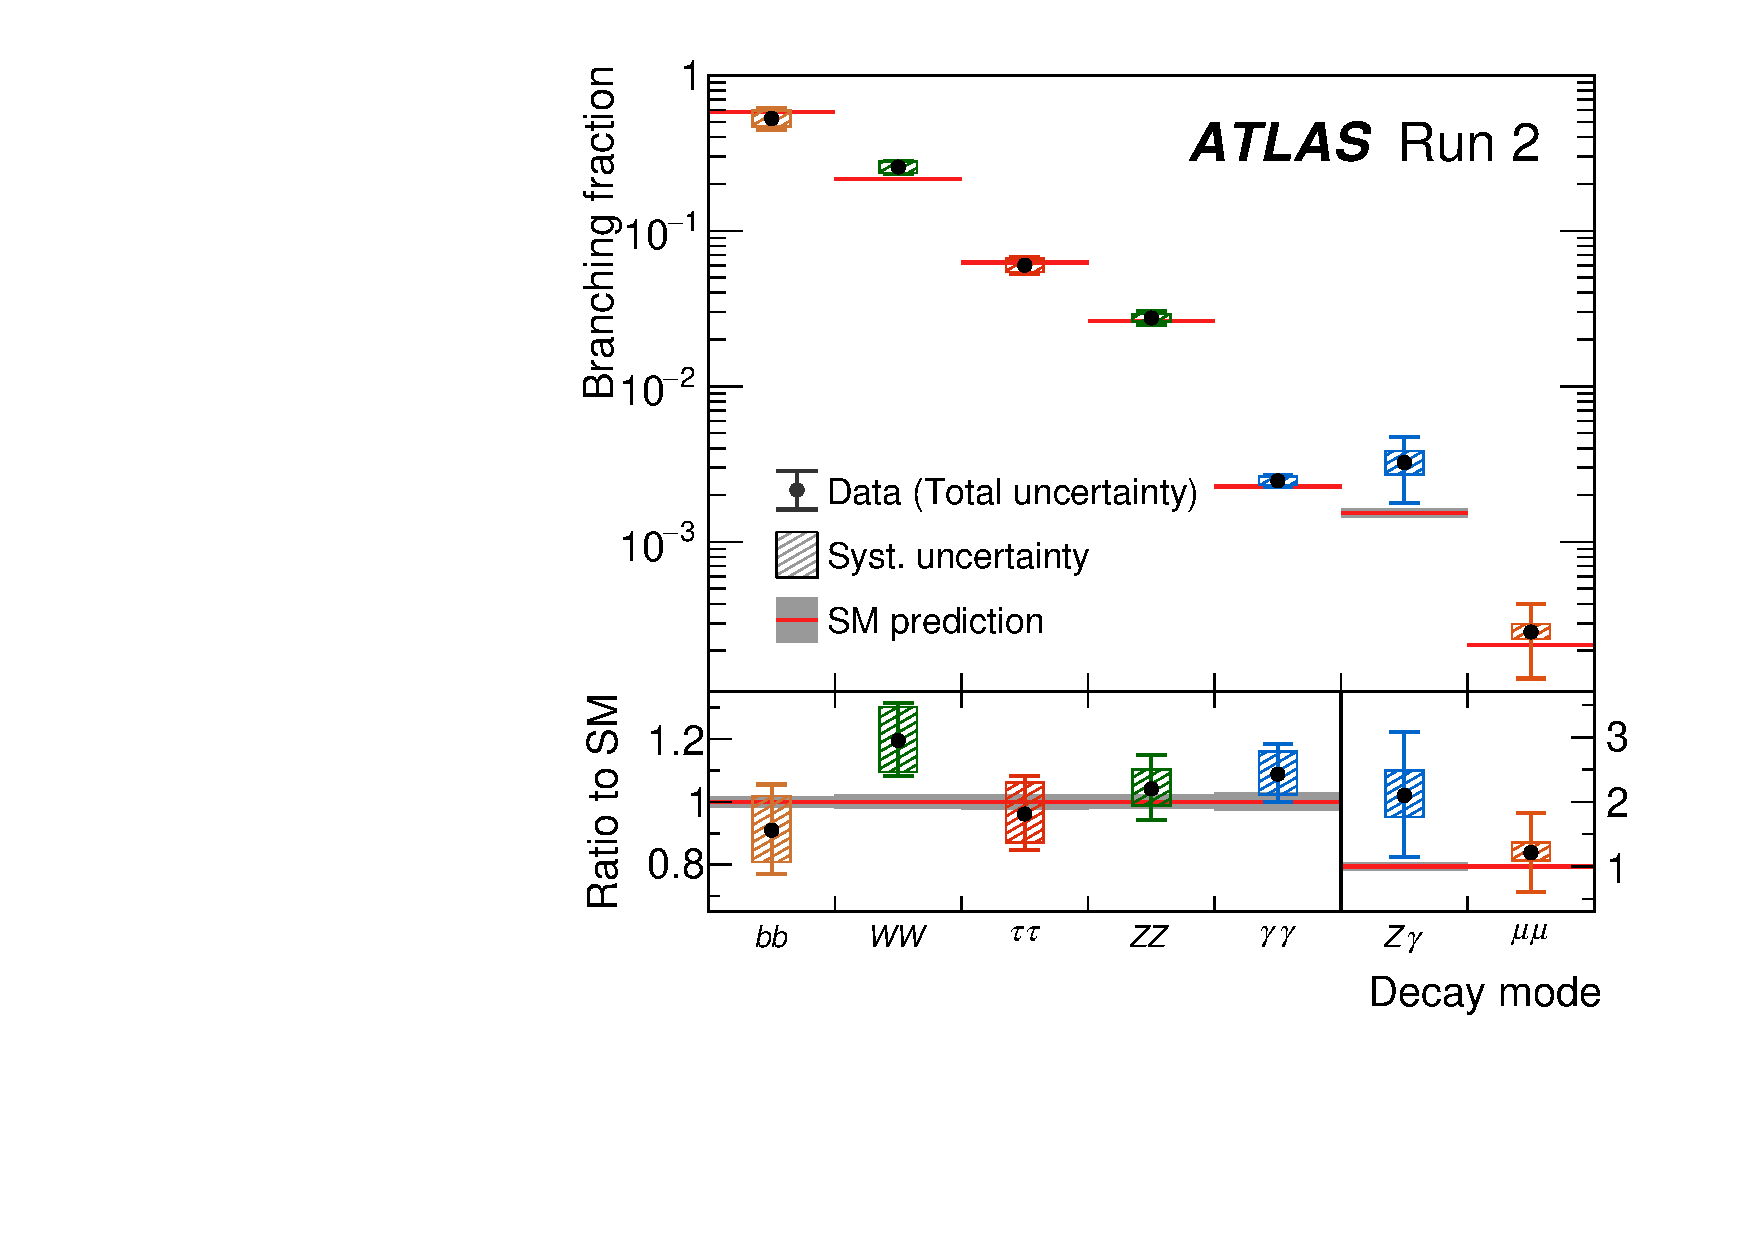
\includegraphics[width=0.48\textwidth]{SM/BRH.pdf}}
        \caption{
            Observed and predicted Higgs boson production cross-sections for different production processes (a) and for different decay modes (b). The lower panels show the ratios of the measured values to their SM predictions. The vertical bar on each point denotes the 68\% confidence interval. The p-value for compatibility of the measurement and the SM prediction is 65\% (a) or 56\% (b)~\cite{HiggssumaryAtlas2022}. 
    }
    \label{figSM:xsecBRH}
    \end{center}
\end{figure}

\clearpage
\subsection{Top quark physics}

The top quark is the most massive known elementary particle, discovered in 1995 at Fermilab~\cite{topsearch1995,PhysRevLett.74.2626}. This characteristic makes the top quark the only one that decays before hadronisation and hence, properties like the spin are directly transferred to the decay products. The main top quark decay is $t\to Wb$ with a branching ratio close to 1, determined by the $V_{tb}=0.97401 \pm 0.00011$ (element of the CKM matrix~\cite{pdg}) being very close to 1. Due to its high mass, the top quark strongly couples with the Higgs boson as the Yukawa coupling (Equation~\ref{Theory_eq:yukawacouplings}) $y_t=\sqrt{2}m_t/v\simeq 1$.\\

Altogether, the top quark plays a key role in the study of the \acrshort{SMlabel}. The precise measurements of its properties put the theory to test and any deviation would point to new physics. It is also an excellent candidate for searches involving either much more massive particles that might decay to the top quark, or decay into other lighter exotic particles. Even if these new particles are too heavy to be produced at the \acrshort{LHClabel}, they can still be detected indirectly through their effects on the properties of the top quark. This makes the top quark an important tool for searching for new physics beyond the \acrshort{SMlabel}. The top quark can be produced either in top quark pairs, namely \ttbar\ production, or together with other particles, called single-top production.\\ % The \ttbar\ production mainly involves the strong interaction and the main Feynman diagrams are shown in Figure\todo{qq->ttbar, gg->ttbar, crossed, s-channel}\\%~\ref{figSM:feynmanttbar}. 

%\begin{figure}[htbp]
%    \RawFloats
%    \begin{center}
%        4 diagrams here
%        \caption{
%            Leading-order Feynman diagrams of the \ttbar\ %production: $gg\to\ttbar$ and $q\bar{q}\to\ttbar$. 
%    }
%    \label{figSM:feynmanttbar}
%    \end{center}
%\end{figure}

The single-top production has three different channels, which involve electroweak interactions: $t$-channel, from $W$ or gluon fusion; $Wt$-channel, with an associated $W$; and $s$-channel, from $q\bar{q}'\to tb$.\\ % Example Feynman diagrams are shown in Figure\todo{qb->q't tchannel, gb->tW Wt, qq'->tb}%~\ref{figSM:feynmanst}.

%\begin{figure}[htbp]
%    \RawFloats
%    \begin{center}
%        3 diagrams here
%        \caption{
%            Examples of leading-order Feynman diagrams of the single-top production for the $t-$channel (a), $Wt-$channel (b) and $s-$channel (c). 
%    }
%    \label{figSM:feynmanst}
%    \end{center}
%\end{figure}

Figure~\ref{figSM:topcrossection} shows a comparison of theoretical and experimental values for the cross-sections involving the production of different top processes, showing an excellent agreement between them. Also, that the \ttbar\ production is larger than the single-top.

\begin{figure}[htbp]
    \RawFloats
    \begin{center}
    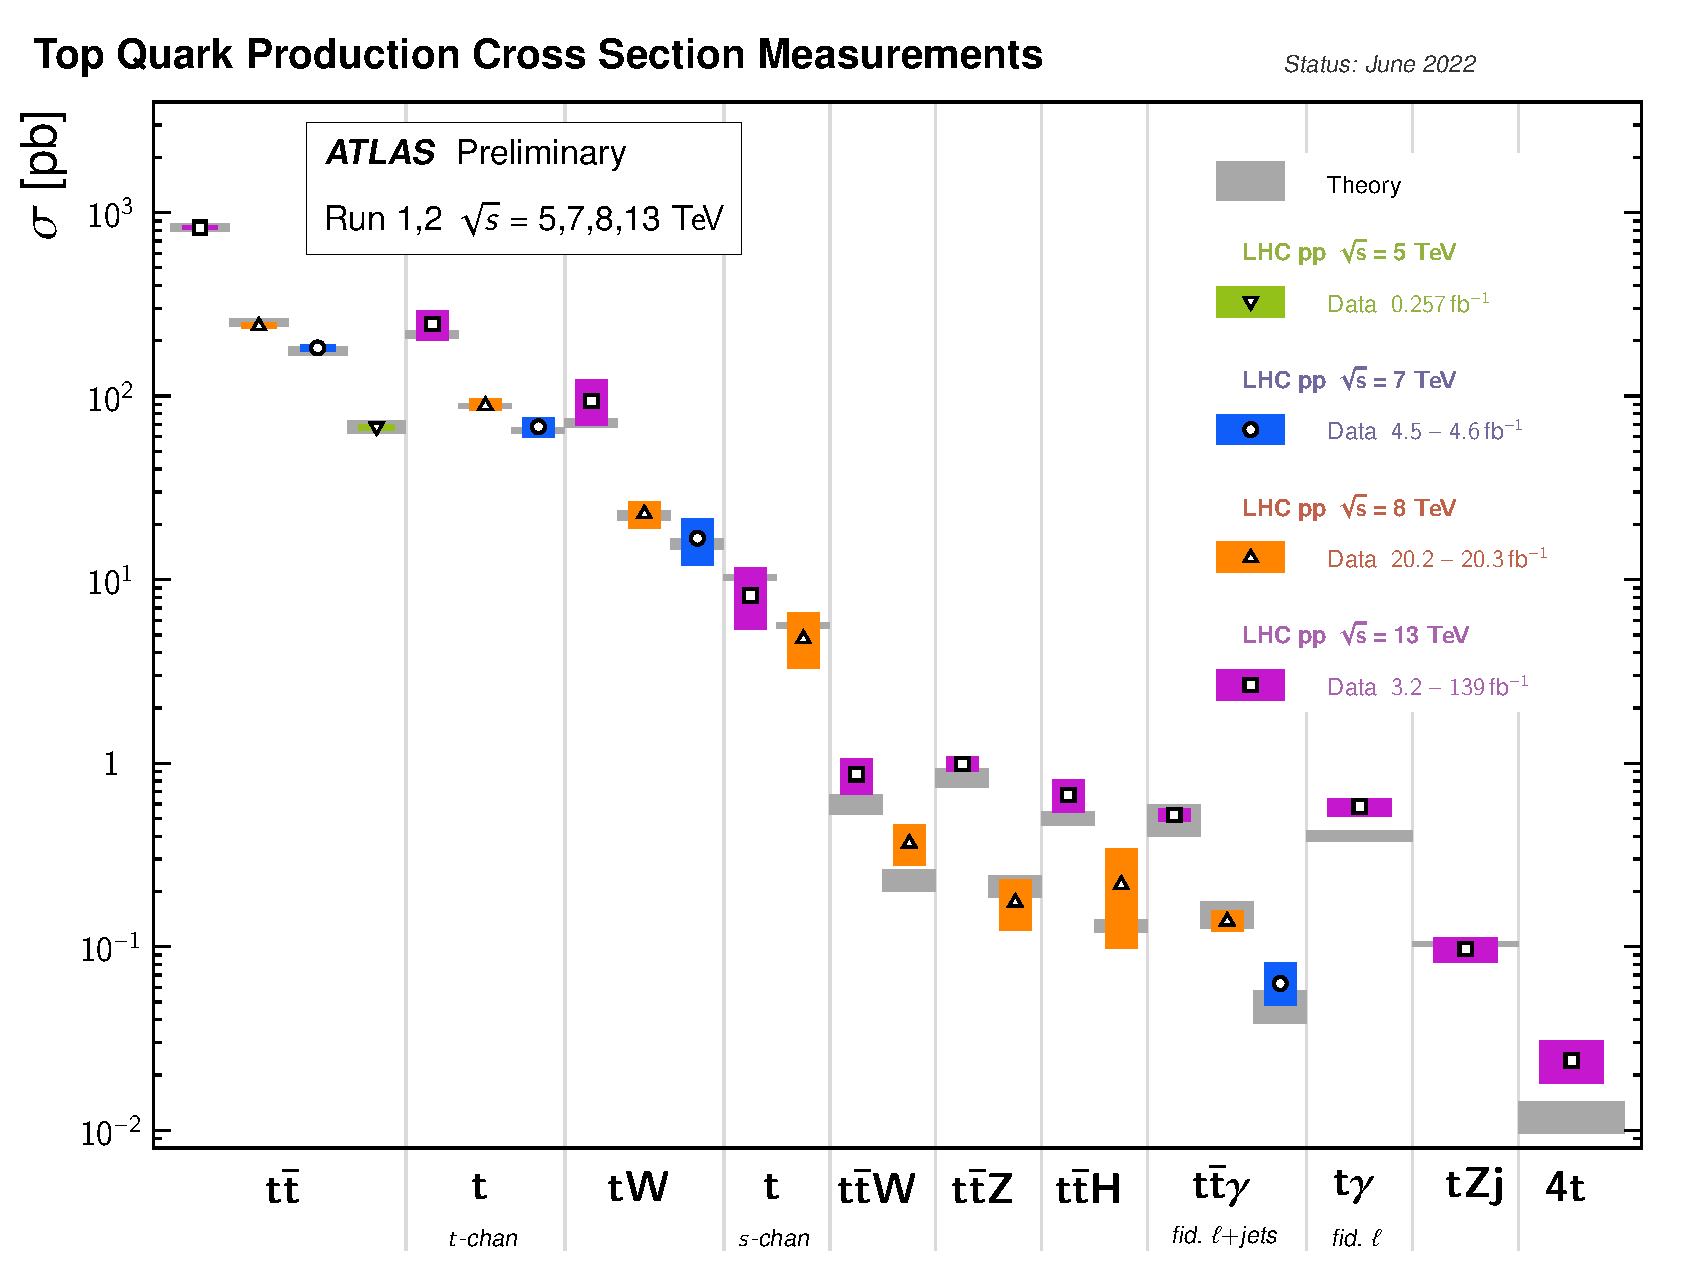
\includegraphics[width=1.0\textwidth]{SM/xsectop.pdf}
    \caption{
        Summary of several top-quark related production cross-section measurements, compared to the corresponding theoretical expectations. All theoretical expectations were calculated at NLO or higher~\cite{ATL-PHYS-PUB-2022-031}.
    }
    \label{figSM:topcrossection}
    \end{center}
\end{figure}

\clearpage
\subsection{FCNC measurements}

A FCNC process stands for an interaction with a change in the fermion (quark or lepton) flavour through
the emission or absorption of a neutral boson. As seen in Section~\ref{Theory_SMsubsec:FCNC}, such processes are not allowed at tree-level in the SM and the one-loop contributions are heavily suppressed by the GIM mechanism.\\

%The FCNC interactions involving the top quark are of particular interest, and the possible diagrams are depicted in Figure\todo{depict tgamam uc, tZ uc, tglu uc, tH uc}.
As the branching ratio of the top quark is mainly $t\to Wb$, together with the heavily suppressed FCNC contributions, the predicted branching ratio for the top FCNC decays in the \acrshort{SMlabel} is below $10^{-14}$. This very small value is far away from the achievable sensitivity at the \acrshort{LHClabel}, and makes the precise measurement of FCNC interactions an excellent test of the \acrshort{SMlabel}.\\

Table~\ref{tabSM:FCNCmeasurements} shows the \acrshort{SMlabel} predictions for all the FCNC top quark decays, together with the experimental results from the \acrshort{SMlabel} and CMS collaborations.

\begin{table}[htbp]
    \addtolength{\leftskip} {-2cm} % menja marges
    \addtolength{\rightskip}{-2cm}
    \begin{tabular}{c|c|cc}
    \toprule\toprule
    Process & \acrshort{SMlabel} & \acrshort{ATLASlabel} & CMS \\ \midrule
    $t\to u\gamma$  & $4\cdot 10^{-16}$ &  $0.85\cdot 10^{-5}$ (139 fb$^{-1}$)  & $1.3\cdot 10^{-4}$ (8~TeV, 19.8 fb$^{-1}$) \\ 
    $t\to c\gamma$  & $5\cdot 10^{-14}$ &  $4.2\cdot 10^{-5}$ (139 fb$^{-1}$)  & $1.7\cdot 10^{-4}$ (8~TeV, 19.8 fb$^{-1}$) \\ \midrule
    $t\to ug$  & $4\cdot 10^{-14}$ &  $0.61\cdot 10^{-4}$ (139 fb$^{-1}$)  & $2.0\cdot 10^{-4}$ (7+8~TeV, 24.7 fb$^{-1}$) \\ 
    $t\to cg$  & $5\cdot 10^{-12}$ &  $3.7\cdot 10^{-4}$ (139 fb$^{-1}$)  & $4.1\cdot 10^{-4}$ (7+8~TeV, 24.7 fb$^{-1}$) \\ \midrule
    $t\to uZ$  & $8\cdot 10^{-17}$ &  $6.2\cdot 10^{-5}$ (139 fb$^{-1}$)  & $2.4\cdot 10^{-4}$ (35.9 fb$^{-1}$) \\ 
    $t\to cZ$  & $1\cdot 10^{-14}$ &  $13\cdot 10^{-5}$ (139 fb$^{-1}$)  & $4.5\cdot 10^{-4}$ (35.9 fb$^{-1}$) \\ \midrule
    $t\to uH$  & $2\cdot 10^{-17}$ &  $6.9\cdot 10^{-4}$ ($H\to\tau\tau$, 139 fb$^{-1}$) & $1.9\cdot 10^{-4}$ ($H\to\gamma\gamma$, 137 fb$^{-1}$) \\ 
    $t\to cH$  & $3\cdot 10^{-15}$ &  $9.4\cdot 10^{-4}$ ($H\to\tau\tau$, 139 fb$^{-1}$) & $7.3\cdot 10^{-4}$ ($H\to\gamma\gamma$, 137 fb$^{-1}$) \\ \midrule
    \bottomrule\bottomrule
    \end{tabular}
    \caption{Theoretical predictions for the branching ratios of FCNC top decays predicted with the \acrshort{SMlabel} \cite{SMFCNC} and the most recent experimental limits from the \acrshort{ATLASlabel}~\cite{ATLAStqgamma,ATLAStqg,ATLAStqHtautau} and the CMS~\cite{CMStqgamma,CMStqg,CMStqZ,CMStqHgammagamma} collaborations.}
    \label{tabSM:FCNCmeasurements}
    \end{table}

\subsection{Open questions}
\label{subsec:openquestions}

The \acrshort{SMlabel} has been successful in describing the fundamental particles and their interactions in nature. However, it is not a complete theory and leaves many open questions about the nature of the universe.\\

One of the most popular issues with the theory is the lack of neutrino mass terms. The observation of neutrino oscillations~\cite{neutrinoosc}  implies the existence of mass differences between the three neutrino generations, but the~\acrshort{SMlabel} does not account for this directly. Different approaches have been proposed, such as adding right-handed neutrinos or describing neutrinos as Majorana particles~\cite{Majorana2006}. However, the~\acrshort{SMlabel} would require at least seven additional parameters: three neutrino masses, three mixing angles and one CP violating phase for the Pontecorvo-Maki-Nakagawa-Sakata (PMNS) matrix~\cite{10.1143/PTP.28.870,Pontecorvo:1967fh}, the neutrino mixing matrix similar to the CKM quark flavour matrix.\\

Another open question concerns the anomalous magnetic dipole moment of the muon. The high-order corrections from~\acrshort{QCD} that appear in this quantity are in tension with the prediction of the~\acrshort{SMlabel}. In 2021, the muon g-2 experiment found a greater deviation~\cite{PhysRevLett.126.141801} from the prediction, highlighting this discrepancy even further.\\

%Other measurements that are in tension with the \acrshort{SMlabel} predictions are regarding the lepton universality, which is the prediction that charged leptons have identical electroweak interaction strenghts. However, the LHCb collaboration found in 2021~\cite{lhcbleptonviolation} a discrepancy between electrons and muons in decays involving the $b-$quark. An older puzzle is the measurement of the anomalous magnetic dipole momentum of the muon, which was found also in tension with the prediction. This quantity refers to the high order corrections that appear from \acrshort{QCD}, and the muon g-2 experiment found a greater deviation~\cite{PhysRevLett.126.141801} in 2021.

The~\acrshort{SMlabel} also fails to describe the other fundamental force in nature: gravity. While general relativity has provided a good description of gravity in macroscopic systems, there is no renomalisable quantum field theory for gravity, and the~\acrshort{SMlabel} does not account for it. Theoretical frameworks like string theory have been proposed as alternatives, but these are difficult to test experimentally. The~\acrshort{SMlabel} is understood as an effective theory of a more complete unified theory and is only valid at low energies. In the most extreme scenario, the~\acrshort{SMlabel} is expected to break around the Planck scale ($M_P=\sqrt{\bar{h}/(8\pi G_N)}\sim 2.4\ 10^{18}$~GeV), where gravitational effects are expected to become as important as the other forces in the \acrshort{SMlabel}.\\

Furthermore, the \acrshort{SMlabel} only describes what is known as baryonic matter, which accounts for about 5\% of the energy density of the universe. Cosmological observations suggest the existence of large amounts of \textit{dark matter} (DM) and \textit{dark energy}, phenomena not accounted for by the \acrshort{SMlabel}. The existence of DM was postulated as extra non-luminous matter needed to explain the clustering of galaxies~\cite{Zwicky2009}. Rotation curves of galaxies not matching the gravitational pull of observed stars~\cite{1981AJ.....86.1825B} and gravitational lensing effects observed in some galaxy collisions~\cite{Umetsu_2016} also provide evidence for large concentrations of invisible mass. More recently, the WMAP and Planck collaborations have studied anisotropies in the cosmic microwave background (CMB)~\cite{Bennett_2013,Planckcollab} and postulated the existence of cold DM. Meanwhile, observations suggest that the universe is expanding at an accelerated rate, compatible with the existence of dark energy, understood to be the product of an intrinsic space-time energy density or cosmological constant that causes the expansion. Observation of the red-shift of light from supernovae, used as standard candles, indicates that cosmological objects are moving away at an increasingly faster rate with the distance~\cite{1929PNAS...15..168H}. Studies of the CMB provide additional measurements of the accelerated expansion~\cite{Planckcollab}. Overall, baryonic matter accounts for only 4.9\% of the total energy density of the universe, dark matter for 26.8\% and dark energy for 68.3\%~\cite{Planckcollab}.\\

The universe appears to be composed entirely of matter. However, to explain the observed imbalance in the abundance of matter and anti-matter, referred to as matter/anti-matter asymmetry, the \acrshort{SMlabel} only provides one source of CP violation in the quark weak interactions, which is not sufficient. Additional sources, such as the complex phase in the PMNS matrix have been proposed. However, it is clear that more phenomena are needed to account for the current net balance of matter. Possible baryon number-violating effects at high energy scales may have played a role in generating this imbalance.\\

Besides the natural phenomena uncovered by the \acrshort{SMlabel}, there are also naturalness problems, which are aesthetic concerns regarding the precise values of some of the \acrshort{SMlabel} parameters. These values seem "unnatural" if there is no underlying mechanism to explain them. The general consensus is that a theory is more natural if it requires fewer fine-tunings. Although these issues are completely subjective, they could be a hint for the existence of a new underlying mechanism that complements the \acrshort{SMlabel}.\\

The first problem, commonly known as the hierarchy problem, arises because the cutoff energy of the \acrshort{SMlabel} ($\Lambda_{\text{SM}}$) is usually set to the Planck scale, $\sim10^{18}$~GeV, whereas the \acrshort{EW} scale ($v\sim246$~GeV) is much smaller. This problem can be understood as the lack of a clear reason why the \acrshort{EWSB} occurs at a sclae orders of magnitude smaller than the Plank scale. High-order corrections from the \acrshort{SMlabel} suggest that the leading radiation corrections for fermion masses are of the order of $\log\Lambda_{\text{SM}}$ and thus sensitive to the scale, but the fine-tuning is considered small. On the other hand, the physical Higgs mass including radiation corrections, is given by,

\begin{equation}
    m^2_H = m_0^2 + \frac{3}{8\pi^2v^2}\Lambda_{\text{SM}}^2 [ m_0^2 + 2m_W^2 + M_Z^2 - 4m_t^2] + \mathcal{O}(\ln\frac{\Lambda_{\text{SM}}}{m_0})
\end{equation}

with $m_0$ the bare Higgs mass. The nature of the hierarchy problem is evident as the correction is more sensitive to the cutoff scale and requires substantial tuning to counter the $\Lambda_{\text{SM}}$ term and achieve such a low measured physical mass. It can also be observed that the most important correction is given by the top quark, and it is often questioned whether the reason for the huge mass of this quark could provide a solution. Although the Higgs mass and the \acrshort{EW} scale are difficult to justify, it can be argued that the appearance of the $\Lambda_{\text{SM}}$ is related to the chosen regularisation scheme, and cutoffs play no physical role.\\

Another related problem is the fermion mass hierarchy; the fact that the masses of the SM particles range from $\sim$1~MeV to $\sim$173~GeV is not understood. Similarly, there is no clear reason for the existence of the three mass families of quarks and leptons with different mixing patterns, with FCNC interactions being heavily suppressed. This problem is known as the flavour problem and might also be related to renormalisation, as fermion masses also have correction terms with the logarithm of the cutoff scale.\\

Another naturalness problem is the strong CP problem, which is related to~\acrshort{QCD}. The most general QCD Lagrangian can contain a CP-violating angle that does not break any symmetry or the renormalisability of the theory. This term would introduce a prediction of axion particles and the neutron having non-zero electric dipole moment. However, the experimental measures of ultracold neutrons and mercury have constrained the CP-violating term to be very small, $\abs{\theta}<6\cdot10^{-11}$~\cite{PhysRevLett.124.081803}, which is an incredibly low value for a parameter that could have any value in the theory. The problem suggests that there may be a yet-unkown symmetry or mechanism that cancels out the CP-violating term.